\documentclass[conf]{new-aiaa}
%\documentclass[journal]{new-aiaa} for journal papers
\usepackage[utf8]{inputenc}

\usepackage{graphicx}
\usepackage{amsmath}
\usepackage{commath}
\usepackage[version=4]{mhchem}
\usepackage{siunitx}
\usepackage{longtable,tabularx}
\usepackage{float}
\usepackage{listings}
\usepackage{pdfpages}
\usepackage{color} %red, green, blue, yellow, cyan, magenta, black, white
\definecolor{mygreen}{RGB}{28,172,0} % color values Red, Green, Blue
\definecolor{mylilas}{RGB}{170,55,241}
\setlength\LTleft{0pt} 

\lstset{language=Matlab,%
	basicstyle=\footnotesize,
	breaklines=true,%
	morekeywords={matlab2tikz},
	keywordstyle=\color{blue},%
	morekeywords=[2]{1}, keywordstyle=[2]{\color{black}},
	identifierstyle=\color{black},%
	stringstyle=\color{mylilas},
	commentstyle=\color{mygreen},%
	showstringspaces=false,%without this there will be a symbol in the places where there is a space
	numbers=left,%
	numberstyle={\tiny \color{black}},% size of the numbers
	numbersep=9pt, % this defines how far the numbers are from the text
	emph=[1]{for,end,break},emphstyle=[1]\color{red}, %some words to emphasise
	%emph=[2]{word1,word2}, emphstyle=[2]{style},    
}

% ================================================================ % 
\title{ASE387P.2 Mission Analysis and Design \\ Homework 3}

\author{Junette Hsin}
\affil{Masters Student, Aerospace Engineering and Engineering Mechanics, University of Texas, Austin, TX 78712}

\begin{document}

\maketitle

% \begin{abstract}

	% Theory and algorithms 

% \end{abstract}

% \newpage 
% ================================================================ % 
\section*{Problem 1}


% ------------------------- % 
\subsection*{A}

To calculate the synodic period, first, the period of Mars was calculated in years: 

\begin{equation}
    T_{Mars} = \frac{1}{\dot{L}_{Mars}} \times \frac{100 \; years}{1 \; century} \times \frac{360 ^\circ}{1 \; rev}
\end{equation}

The synodic period was then calculated with the following equation: 

\begin{equation}
    SP_{Mars} = \frac{T_{Mars}}{|| T_{Mars} - 1 ||}
\end{equation}

The synodic period came out to be 2.13526965089401. 

% ------------------------- % 
\subsection*{B}

\textbf{All analyses for this section are for a desired 60 degree transfer angle in the clockwise direction from the initial / departure position.} \\ 

The desired transfer angle of 60 degrees was defined to be the angle between the initial / departure longitude and the final / arrival longitude. 

\begin{equation}
    \Delta L_{des} = L_{M_f} - L_{E_i}
    \label{eq:DL}
\end{equation}

For an outbound transfer, the initial longitude would be Earth and the final longitude would be Mars. For inbound transfer, the initial longitude would be Mars and the final longitude would be Earth. Equation \ref{eq:DL} could also be rewritten as: 

\begin{equation}
    L_{M_f} = \Delta L_{des} + L_{E_i}
    \label{eq:Lf1}
\end{equation}

The final longitude can also be found from the motion of the planets: 

\begin{equation}
    L_{M_f} = L_{M_i} + \Delta t \dot{L_{M}}
    \label{eq:Lf2}
\end{equation}

Combing Equations \ref{eq:Lf1} and \ref{eq:Lf2} result in: 

\begin{equation}
    \Delta t = \frac{\Delta L_{des} + L_{E_i} - L_{M_i}}{ \dot{L_M} }
\end{equation}

The document \textbf{aprx\_pos\_planets.pdf} was used to compute the orbital elements and Cartesian states of Earth and Mars. Once $\Delta t$ and an initial time are known, the positions of the planets are known. The Lambert solver from HW 2 was used to find the time of flight for the minimum energy transfer. \\ 

The above algorithm was iterated until the TOF for the minimum energy transfer aligned with the time for a 60 degree transfer angle between departure and arrival positions to develop. For example, for an outbound trajectory from Earth to Mars, the 60 degree transfer angle is computed between the initial Earth position and the final Mars position. Mars will take some amount of time, which we will call $\Delta t_M$, to travel from its initial position at launch date to its final position at the arrival date. The algorithm was iterated until the TOF for the minimum energy transfer aligned with $\Delta t_M$.  \\ 

\textbf{1st Launch Window} \\ 

The launch date (T0), arrival date (T1), and the time of flight for the 1st launch window are displayed in the figure below. \\ 

The longitude orbital elements are: \\ 

E (T0) longitude = 352.527823989418 $^\circ$ \\ 

M (T0) longitude = 320.871016064409 $^\circ$ \\ 

M (T1) longitude = 52.5278239893489 $^\circ$ 

\begin{figure}[H]
    \centering 
    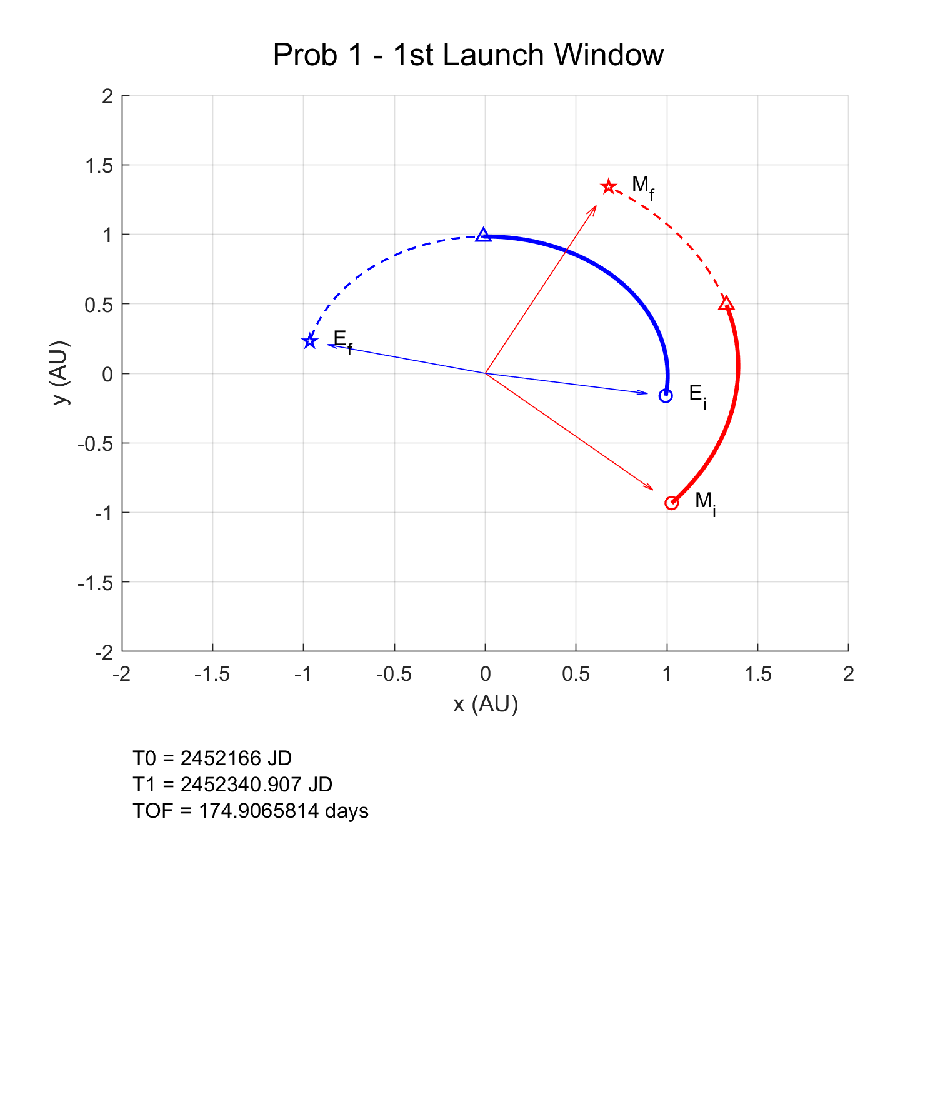
\includegraphics[width=0.7\textwidth]{Prob 1 - 1st Launch Window.pdf}
    \caption{1st Earth to Mars 60 degrees transfer}
\end{figure}

\textbf{2nd Launch Window}

The launch date (T0), arrival date (T1), and the time of flight for the 2nd launch window are displayed in the figure below. \\ 

E (T0) longitude = 51.0669403240372 $^\circ$ \\ 

M (T0) longitude = 14.8080745374352 $^\circ$ \\

M (T1) longitude = 111.066940324018 $^\circ$ 

\begin{figure}[H]
    \centering 
    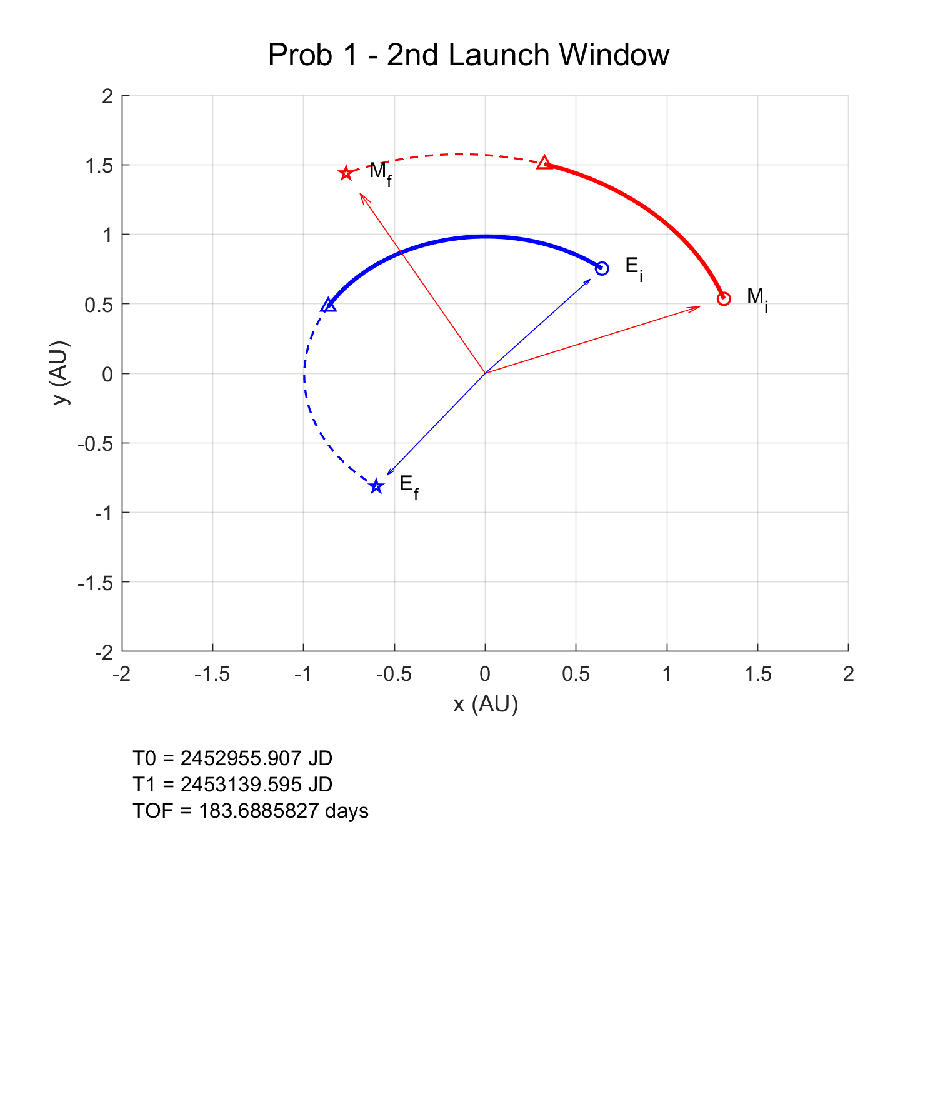
\includegraphics[width=0.7\textwidth]{Prob 1 - 2nd Launch Window.pdf}
    \caption{2nd Earth to Mars 60 degrees transfer}
\end{figure}

% ------------------------- % 
\subsection*{C}

The launch date (T0), arrival date (T1), and the time of flight for the inbound conic are displayed in the figure below. \\ 

E (T0) longitude = 75.1475543810473 $^\circ$ \\

E (T1) longitude = 279.017723434249 $^\circ$ \\

M (T0) longitude = 219.017723434434 $^\circ$ 

\begin{figure}[H]
    \centering 
    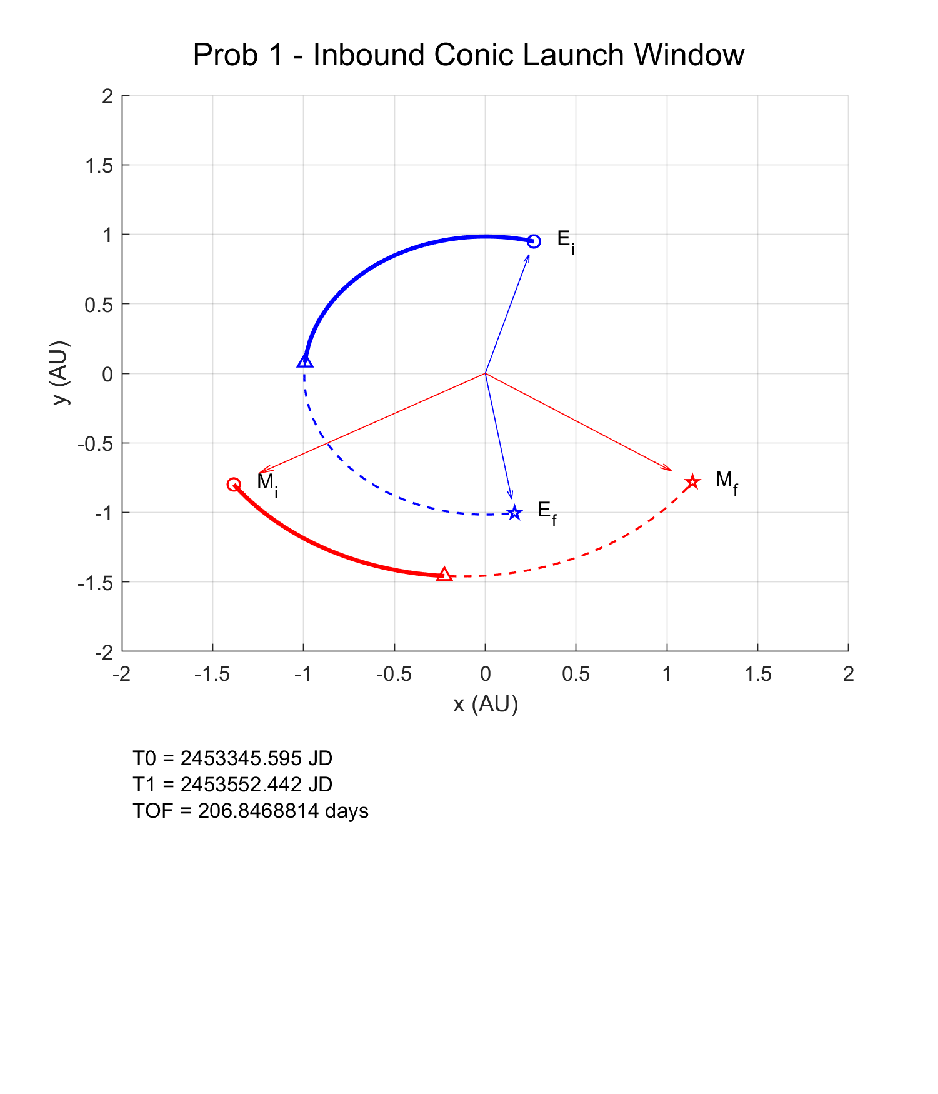
\includegraphics[width=0.7\textwidth]{Prob 1 - Inbound Conic Launch Window.pdf}
    \caption{Inbound Mars to Earth 60 degrees transfer}
\end{figure}

% \newpage 
% ================================================================ % 
\section*{Problem 2}

\subsection*{A}
In the previous section, the angle between Earth and Mars was computed using the approximate longitude from \textbf{aprx\_pos\_planets.pdf}. For Problem 2, the 1.85 $^\circ$ inclination of Mars' orbit was factored into the angle calculation. \\ 

To compute the desired inclination-corrected longitude for Mars, the departure vector, $\overrightarrow{r} _{dep}$ was first rotated 60 degrees about the Earth orbit normal. In the ecliptic frame, this is the same as a rotation about the Z axis:  

\begin{equation}
    \overrightarrow{r}_{rot}  = R_z(60 ^\circ) \overrightarrow{r}_{dep}  
\end{equation}

Then, the rotated vector, $\overrightarrow{r}_{rot} $ was projected onto the Mars orbit normal, $\hat{h}$, which is inclined 1.85 $^\circ$ about the Martian longitude of the ascending node. 

\begin{equation}
    \overrightarrow{r}_{proj,h}  = \frac{ \overrightarrow{r}_{rot}  \cdot \hat{h} }{ ||\overrightarrow{r}_{rot}|| \; ||\hat{h}|| } \hat{h}
\end{equation}

Finally, the projected vector, $\overrightarrow{r} _{proj,h}$ was subtracted from the $\overrightarrow{r} _{rot}$ to obtain the projection of the rotated vector onto the Martian orbital plane, $r_{proj,plane}$, which is also our desired arrival vector, $r_{arr}$. 

\begin{equation}
    \overrightarrow{r}_{arr} = \overrightarrow{r}_{rot} - \overrightarrow{r}_{proj,h}
\end{equation}

The transfer angle between $\overrightarrow{r}_{dep}$ and $\overrightarrow{r}_{arr}$ will either be greater than or less than 60 degrees, depending on whether the Martian orbit normal is inclined toward or away from $\overrightarrow{r}_{dep}$. A minimization routine was then used to augment the rotation angle used to create $\overrightarrow{r}_{rot}$ until the final transfer angle was within a tolerance of 60 degrees. \\ 

The launch date (T0), arrival date (T1), and the time of flight for the 2nd launch window are displayed in the figure below. \textbf{The z axis is zoomed in to show the exaggerated inclination of Mars' orbit.}

\begin{figure}[H]
    \centering 
    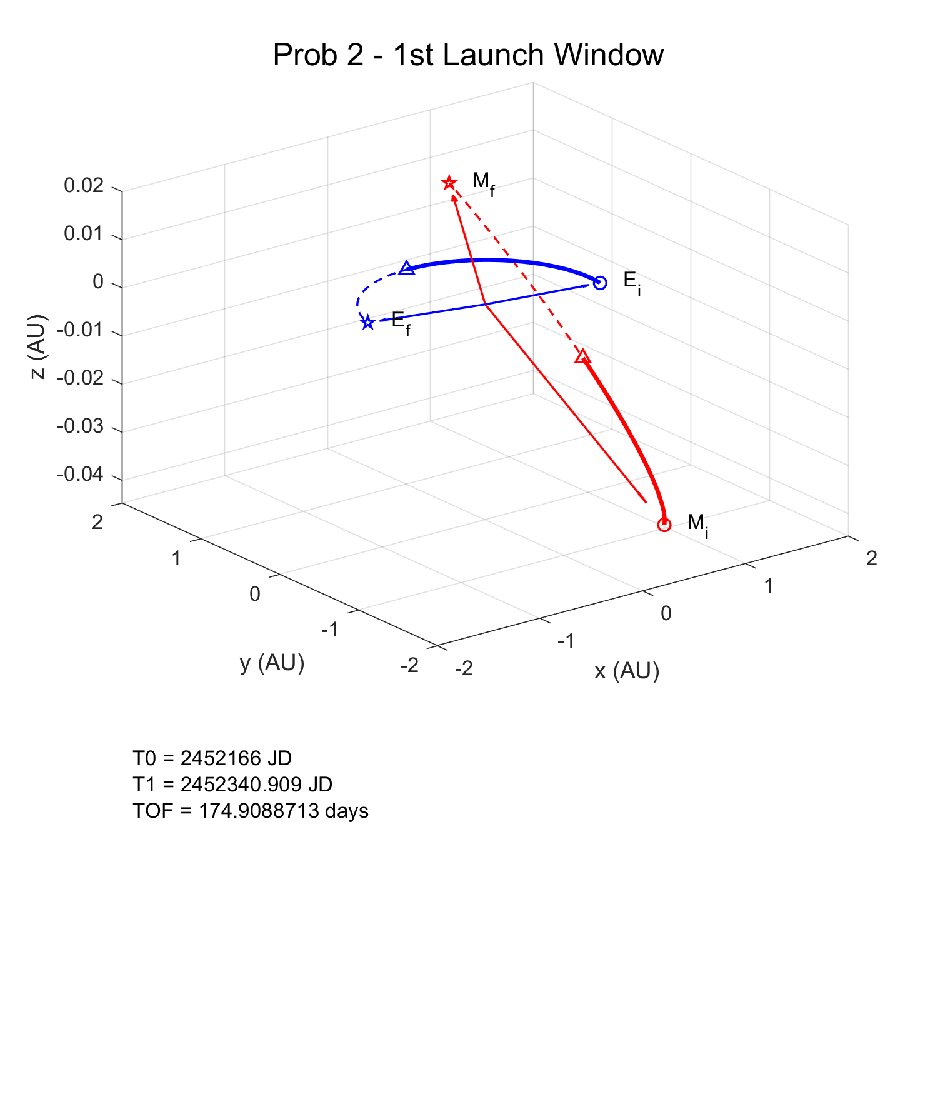
\includegraphics[width=0.7\textwidth]{Prob 2 - 1st Launch Window.pdf}
    \caption{1st Earth to Mars 60 degrees transfer with Mars inclination}
\end{figure}

\begin{figure}[H]
    \centering 
    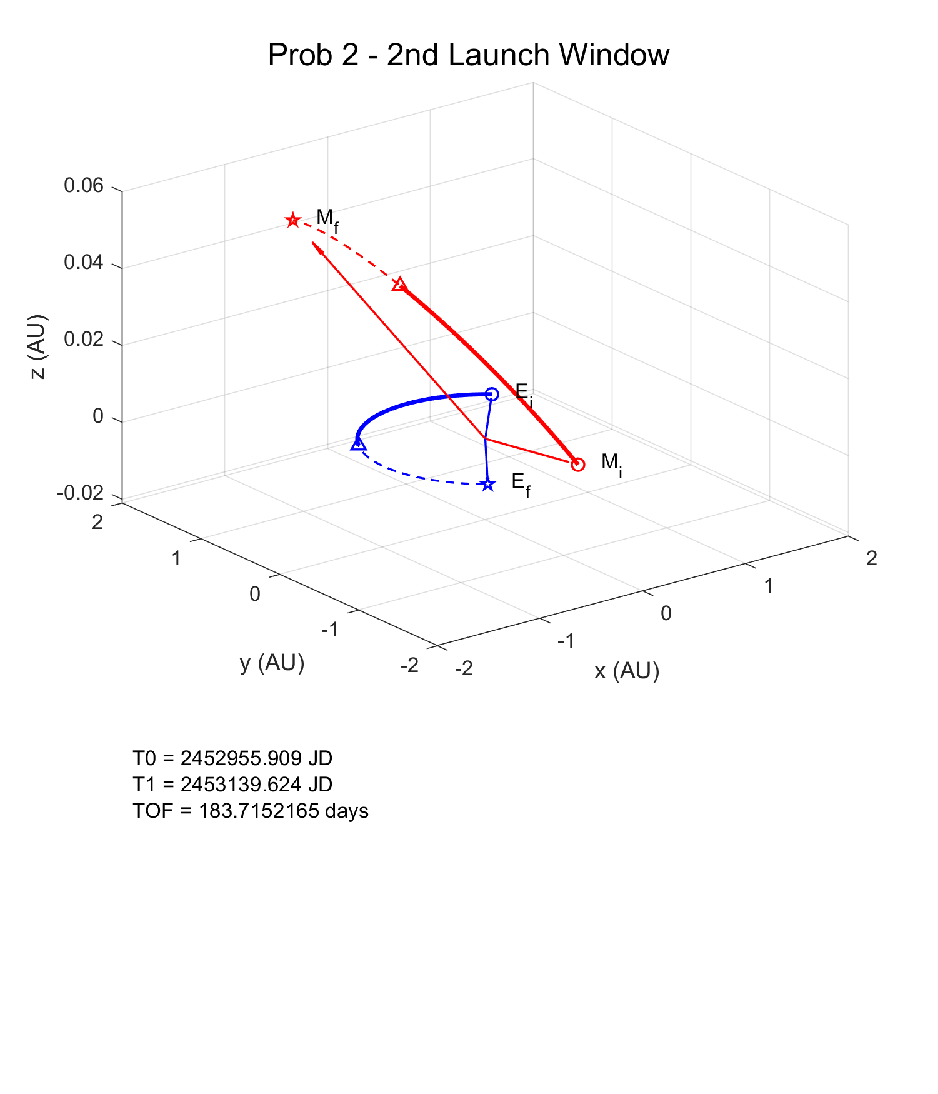
\includegraphics[width=0.7\textwidth]{Prob 2 - 2nd Launch Window.pdf}
    \caption{2nd Earth to Mars 60 degrees transfer with Mars inclination}
\end{figure}

\begin{figure}[H]
    \centering 
    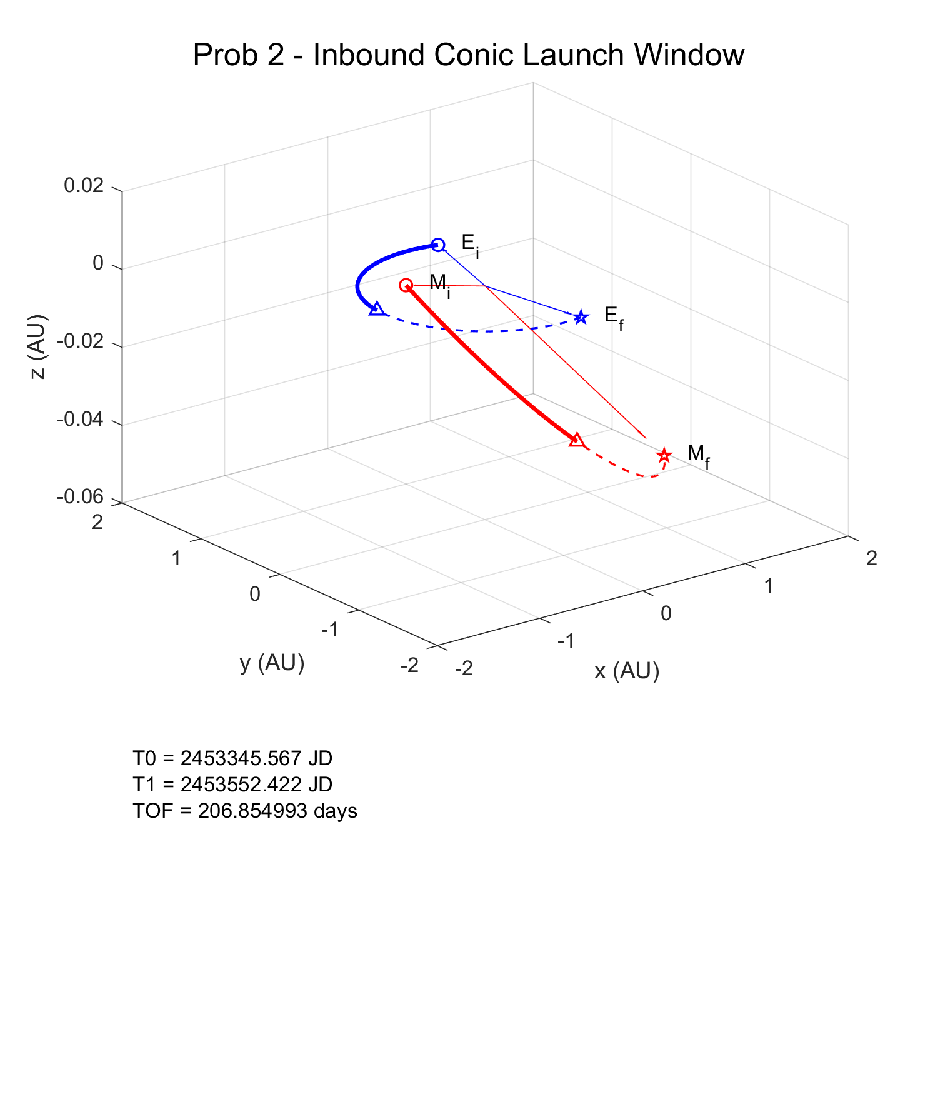
\includegraphics[width=0.7\textwidth]{Prob 2 - Inbound Conic Launch Window.pdf}
    \caption{Inbound Mars to Earth 60 degrees transfer with Mars inclination}
\end{figure}

% ------------------------- % 
\subsection*{B}

For the 1st launch window, the Martian longitude at the arrival point is 52.529023989479 $^\circ$. In Problem 1, the longitude is 52.5278239893489 $^\circ$. That is a difference of 0.00120000013009758 $^\circ$. \\ 

For the 2nd launch window, the Martian longitude at the arrival point is 111.082097302582 $^\circ$. In Problem 1, the longitude is 111.06694032401 $^\circ$. That is a difference of 0.0151569785719943 $^\circ$. \\ 

For the inbound conic, the Earth longitude at the arrival point is 279.030980413165 $^\circ$. In Problem 1, the longitude is 279.017723434249 $^\circ$. That is a difference of 0.013256978916047 $^\circ$. 

% ================================================================ % 
% Problem 3 

\section*{Problem 3}

% ------------------------- % 
\subsection*{A}

The Earth SOI was found to be 924644.363478889 km. \\ 

The Mars SOI was found to be 577259.24645827 km. Plots for the central and perturbing accelerations for the entire transfer duration as well as in the vicinity of the SOI are given below. 

\begin{figure}[H]
    \centering 
    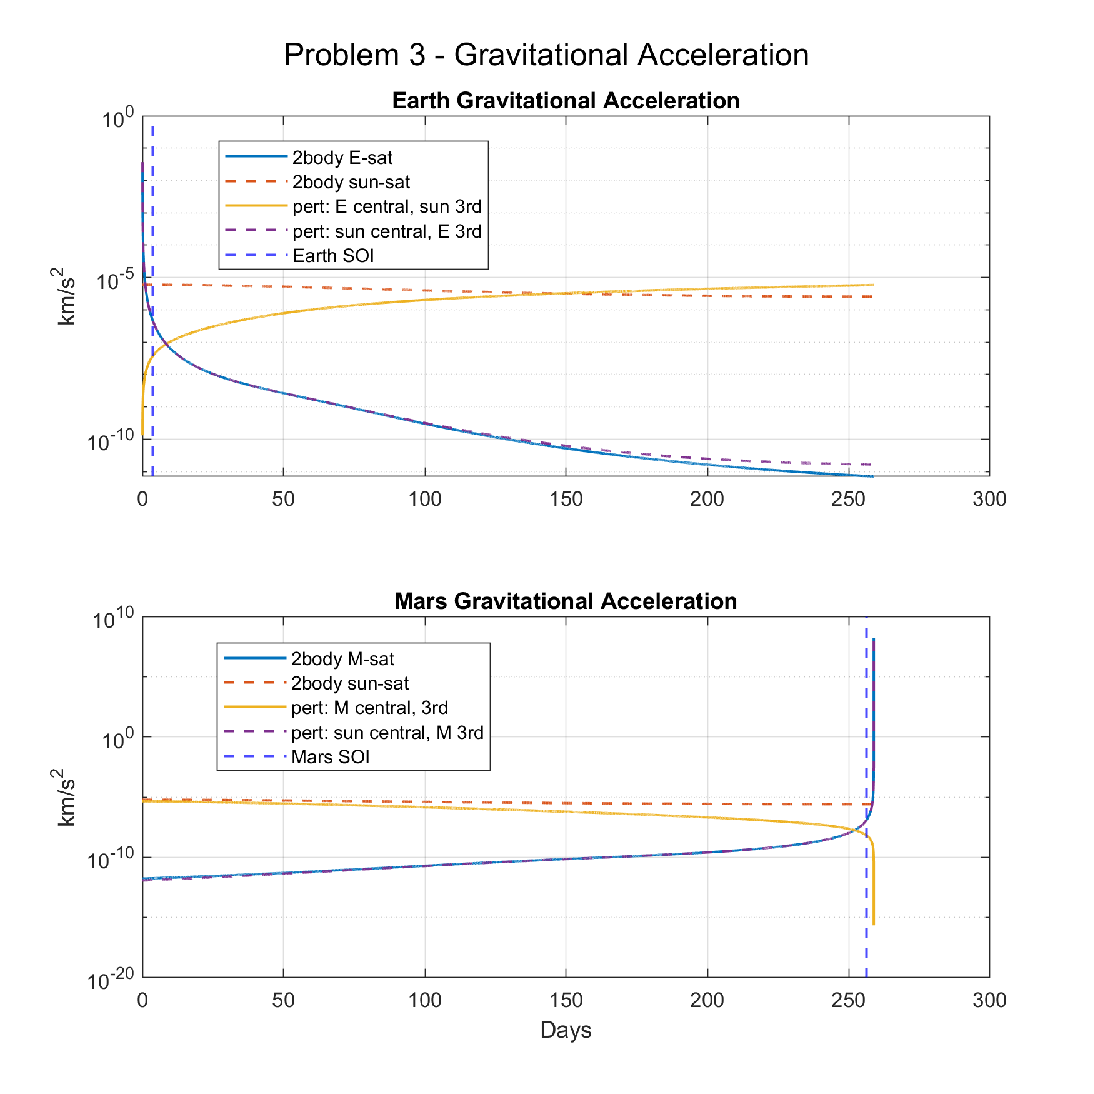
\includegraphics[width=0.7\textwidth]{Problem 3 - Gravitational Acceleration.pdf}
    \caption{Gravitational acceleration}
\end{figure}

\begin{figure}[H]
    \centering 
    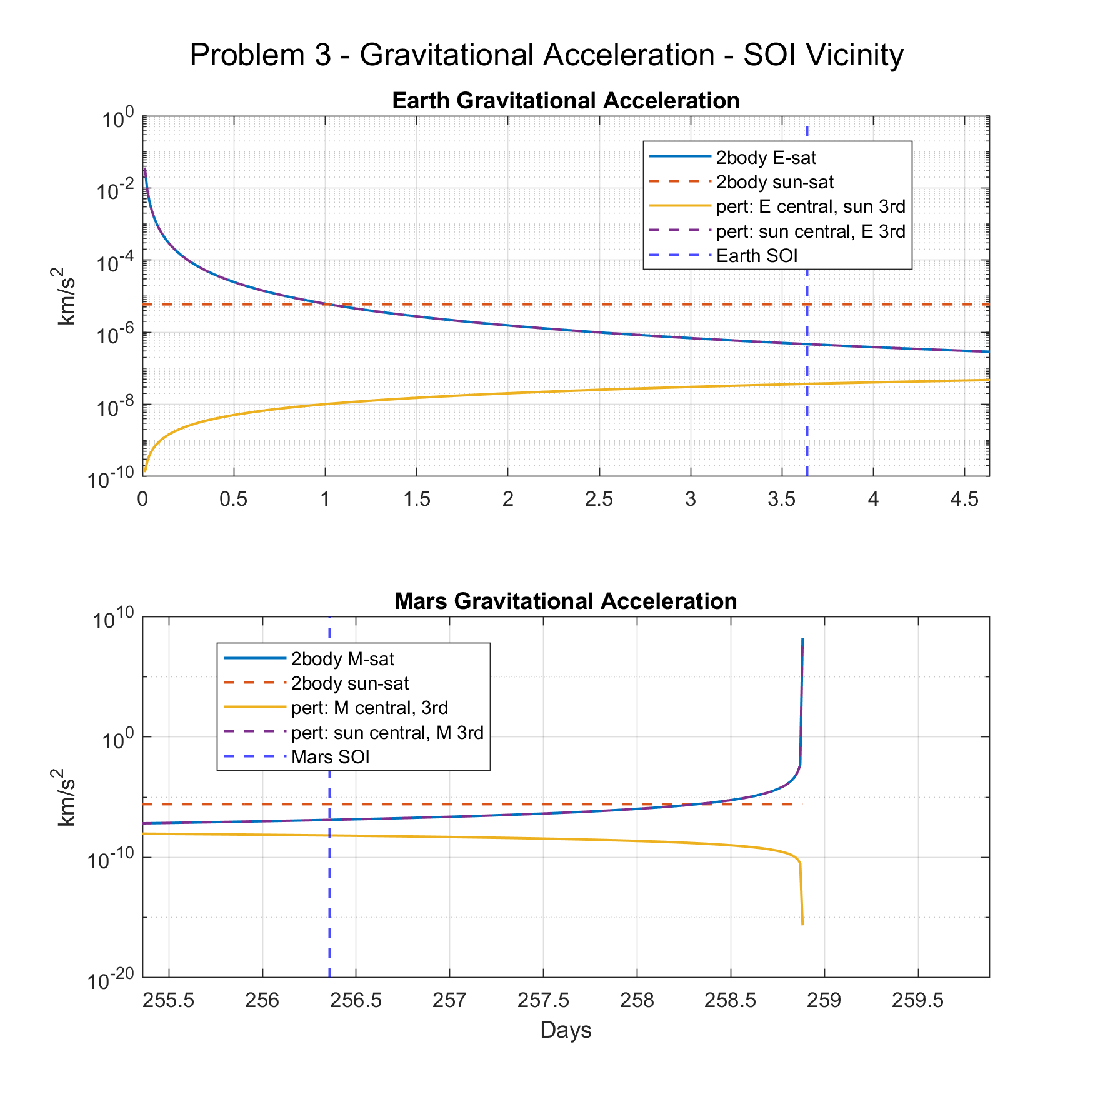
\includegraphics[width=0.7\textwidth]{Problem 3 - Gravitational Acceleration - SOI Vicinity.pdf}
    \caption{Gravitational acceleration - SOI Vicinity}
\end{figure}


% ------------------------- % 
\subsection*{B}

Plots for the ratios and rate of change of central to perturbing accelerations for the entire transfer duration as well as in the vicinity of the SOI are given below. \\ 

Figure \ref{fig:accel_ratio_SOI} shows the ratios in the vicinity of the SOIs. The location to patch the conics should be applied at the edge of the sphere of influence. By considering only the gravitational force between the spacecraft and the body whose sphere of influence is considered, complicated N-body problems can be reduced to 2-body problems. Once the spacecraft is out of the smaller body's sphere of influence, then the gravitational force between the spacecraft and the larger body is used for trajectory calculations. 

\begin{figure}[H]
    \centering 
    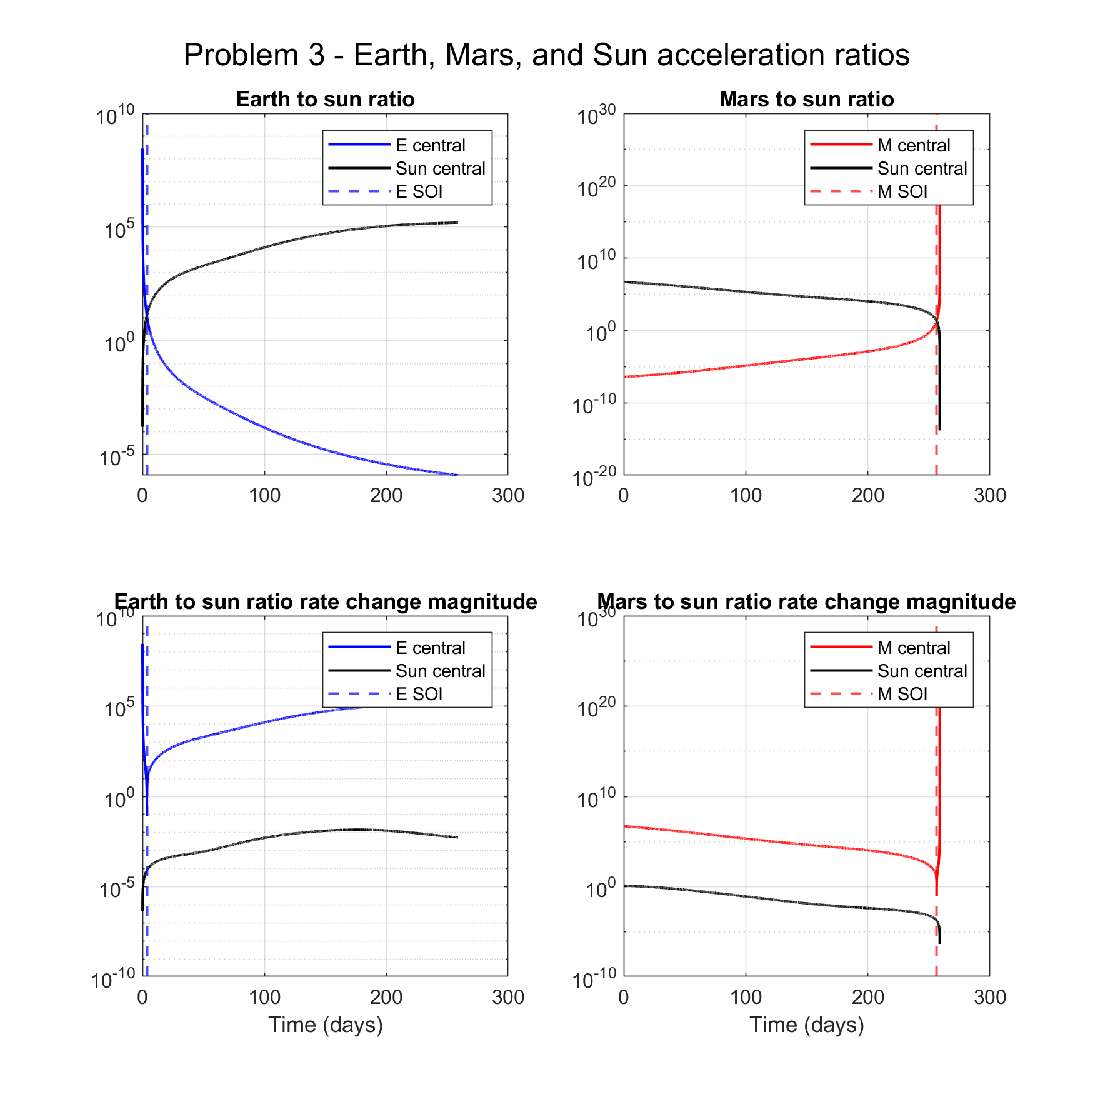
\includegraphics[width=0.7\textwidth]{Problem 3 - Earth, Mars, and Sun acceleration ratios.pdf}
    \caption{Gravitational acceleration ratios}
\end{figure}

\begin{figure}[H]
    \centering 
    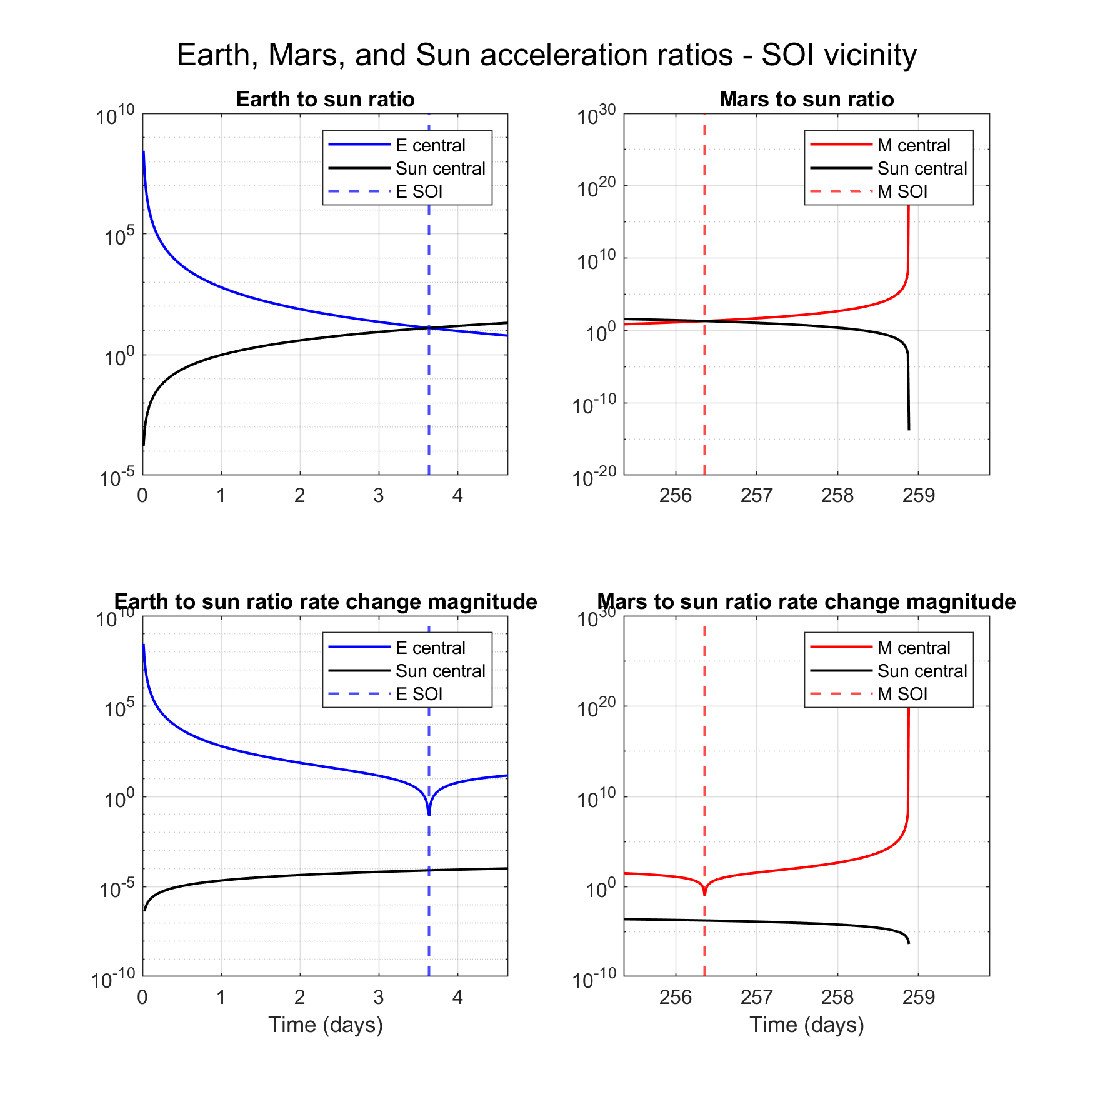
\includegraphics[width=0.7\textwidth]{Problem 3 - Earth, Mars, and Sun acceleration ratios - SOI vicinity.pdf}
    \caption{Gravitational acceleration ratios - SOI Vicinity}
    \label{fig:accel_ratio_SOI}
\end{figure}

% ------------------------- % 
\subsection*{C}

The flight path angle is needed to compute the conditions for capture upon entering a planet's sphere of influence. The true anomaly and delta-V required for the capture burn can be calculated from the flight path angle. \\ 

The flight path angle is also used to comptue the conditions for leaving the sphere of influence. The fly-by heliocentric orbit uses the flight path angle to calculate the angular momentum as well as the spacecraft true anomaly in its heliocentric orbit. 

\begin{figure}[H]
    \centering 
    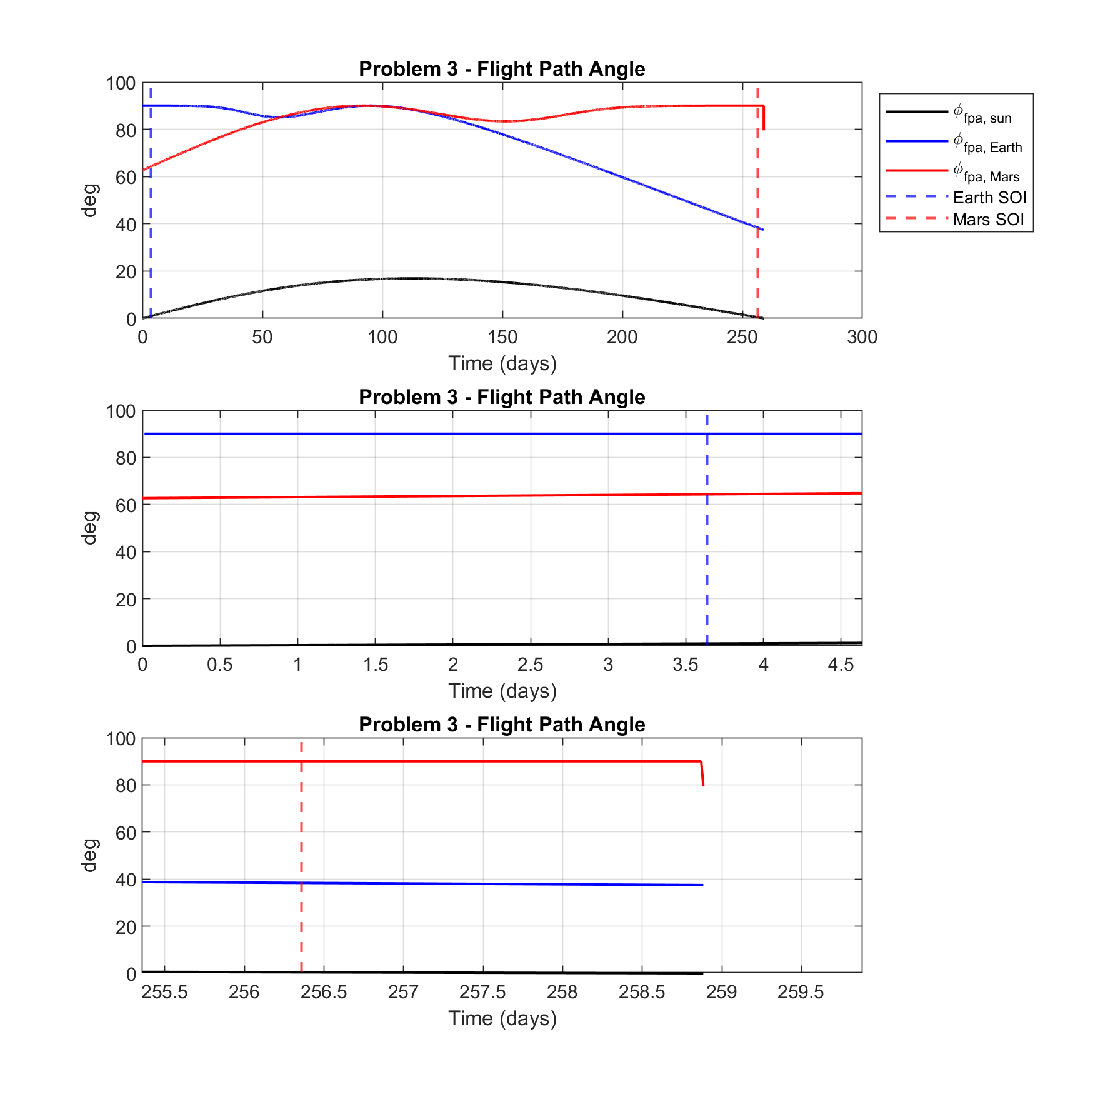
\includegraphics[width=0.7\textwidth]{Problem 3 - Flight Path Angle.pdf}
    \caption{Flight Path Angle}
\end{figure}


% ================================================================ % 
% Problem 4 

\section*{Problem 4}

% ------------------------- % 
\subsection*{A}

The separation distance is calculated: 

\begin{equation}
    \Delta = \sqrt{\frac{e + 1}{e - 1}} 
\end{equation}

The eccentricity is calculated from: 

\begin{equation}
    e = 1 + \frac{r_p v_{inf}^2}{\mu}
\end{equation}

The turning angle can also be calculated from eccentricity: 

\begin{equation}
    \phi = 2 sin^{-1} \frac{1}{e}
\end{equation}

$\Delta v$ can be calculated from: 

\begin{equation}
    \Delta \overrightarrow{v} = \overrightarrow{v}_f - \overrightarrow{v}_i
\end{equation}

$\overrightarrow{v}_f$ is a function of the turning angle and planet velocities: 

\begin{equation}
    \overrightarrow{v}_f = R_x(\phi) ( \overrightarrow{v}_i - \overrightarrow{v}_p ) + \overrightarrow{v}_p
\end{equation}

% ------------------------- % 
\subsection*{B}

To alter the transfer conic and phasing from the gravity-assist fly-by, the turning angle $\phi$ and the $\Delta v$ must be added to the orbit. If the planet does not intersect with the target planet with the  added velocity, then there is a possibility that no valid solution exist at the current phasing with the given entrance velocity. To change the entrance velocity or improve phasing, one could start the interplanetary trajectory design with the lowest possible flyby distance. If a solution is still not reached, then increment the distance or increase the time for a different phasing. 

% \newpage
% ================================================================ % 
\section*{Appendix} 

\subsection*{MATLAB code} 

\begin{lstlisting}

    %% HW 2 
    % Junette Hsin 
    
    % Keplerian elements 
    % a     = semi-major axis 
    % e     = eccentricity 
    % i     = inclination 
    % L     = mean longitude 
    % wbar  = longitude of perihelion 
    % Omega = longitude of ascending node 
    
    clear; clc 
    
    % Earth 
    Earth.a0 =      1.00000261; 
    Earth.da =      0.00000562; 
    Earth.e0 =      0.01671123; 
    Earth.de =     -0.00004392; 
    Earth.I0 =     -0.00001531; 
    Earth.dI =     -0.01294668;
    Earth.L0 =    100.46457166; 
    Earth.dL =  35999.37244981; 
    Earth.wbar0 = 102.93768193; 
    Earth.dwbar =   0.32327364;
    Earth.Omega0 =  0; 
    Earth.dOmega =  0; 
    
    % Mars 
    Mars.a0 =      1.52371034; 
    Mars.da =      0.00001847; 
    Mars.e0 =      0.09339410; 
    Mars.de =      0.00007882; 
    Mars.I0 =      1.84969142; 
    Mars.dI =     -0.00813131; 
    Mars.L0 =     -4.55343205 + 360; 
    Mars.dL =  19140.30268499; 
    Mars.wbar0 = -23.94362959; 
    Mars.dwbar =   0.44441088; 
    Mars.Omega0 = 49.55953891; 
    Mars.dOmega = -0.29257343; 
    
    % sun mu (m^3/s^2)
    mu_sun_m = 1.32712440018e20; 
    mu_sun_km = mu_sun_m / (1000^3); 
    mu = mu_sun_km; 
    
    
    %% synodic period 
    
    dL_E = Earth.dL; 
    dL_M = Mars.dL;         % degrees per century 
    
    % period of Earth 
    T_E = 365.25; 
    
    % period of Mars 
    dL_M_degyear = dL_M / 100;      % degs per year
    T_M_years = (1/dL_M_degyear) * 360;            % period (days per 360 deg) 
    
    % synodic period 
    SP_M = T_M_years / abs(T_M_years - 1); 
    
    disp('Synodic period:') 
    disp(SP_M) 
    
    %% find launch date 
    
    T0 = 2451545.0; % units = days 
    
    T = T0;
    [dt_days1, tof1_1, tof1_2] = launch_date(T, Earth, Mars, mu); 
    % find 1st launch date 
    while abs(dt_days1 - tof1_1) > 1 && abs(dt_days1 - tof1_2) > 1
    
        T = T + 1; 
        [dt_days1, tof1_1, tof1_2] = launch_date(T, Earth, Mars, mu); 
        
    end 
    
    % check 
    [r_E0, ~, oe_E0] = xyz_ecl(T, Earth); 
    [r_M0, ~, oe_M0] = xyz_ecl(T, Mars); 
    [r_E1, ~, oe_E1] = xyz_ecl(T + dt_days1, Earth); 
    [r_M1, ~, oe_M1] = xyz_ecl(T + dt_days1, Mars); 
    phi = acosd(dot(r_E0, r_M1) / ( norm(r_E0)*norm(r_M1) ))
    disp('1st launch window: ')
    disp('E0 longitude = ') 
    L_E0 = oe_E0(4)
    disp('M0 longitude = ') 
    L_M1 = oe_M0(4)
    disp('M1 longitude = ') 
    L_M1 = oe_M1(4)
    
    T0 = T; 
    T1 = T0 + dt_days1; 
    
    % ok let's do a propagation ... 
    
    r_E_hist_T0T1 = []; 
    r_M_hist_T0T1 = []; 
    for i = 0 : 0.1 : dt_days1
        
        Ti = T0 + i; 
        
        % Earth 
        [r_E, r_p, oe_E] = xyz_ecl(Ti, Earth); 
        r_E_hist_T0T1 = [r_E_hist_T0T1; r_E']; 
    %     oe_E_hist_T0T1(i+1,:) = oe_E'; 
        
        % Mars 
        [r_M, r_p, oe_M] = xyz_ecl(Ti, Mars); 
        r_M_hist_T0T1 = [r_M_hist_T0T1; r_M']; 
    %     oe_M_hist_T0T1(i+1,:) = oe_M'; 
        
    end 
    
    txt = {sprintf('T0 = %.10g JD', T0); ... 
        sprintf('T1 = %.10g JD', T1); ... 
        sprintf('TOF = %.10g days', dt_days1) ... 
        }; 
    plot3_p1p2(r_E_hist_T0T1, r_M_hist_T0T1, r_E0, r_M0, r_E1, r_M1, 'Prob 1 - 1st Launch Window', txt)
    fn.save_pdf(gcf)
    
    
    %% find 2nd launch date 
    
    T = T1;
    [dt_days1, tof1_1, tof1_2] = launch_date(T, Earth, Mars, mu); 
    % find 1st launch date 
    while abs(dt_days1 - tof1_1) > 1 && abs(dt_days1 - tof1_2) > 1
    
        T = T + 1; 
        [dt_days1, tof1_1, tof1_2] = launch_date(T, Earth, Mars, mu); 
        
    end 
    
    % check 
    [r_E0, ~, oe_E0] = xyz_ecl(T, Earth); 
    [r_M0, ~, oe_M0] = xyz_ecl(T, Mars); 
    [r_E1, ~, oe_E1] = xyz_ecl(T + dt_days1, Earth); 
    [r_M1, ~, oe_M1] = xyz_ecl(T + dt_days1, Mars); 
    phi = acosd(dot(r_E0, r_M1) / ( norm(r_E0)*norm(r_M1) ))
    disp('2nd launch window: ')
    disp('E0 longitude = ') 
    L_E0 = oe_E0(4)
    disp('M0 longitude = ') 
    L_M1 = oe_M0(4)
    disp('M1 longitude = ') 
    L_M1 = oe_M1(4)
    
    T0 = T; 
    T1 = T0 + dt_days1; 
    
    % ok let's do a propagation ... 
    
    r_E_hist_T0T1 = []; 
    r_M_hist_T0T1 = []; 
    for i = 0 : 0.1 : dt_days1
        
        Ti = T0 + i; 
        
        % Earth 
        [r_E, r_p, oe_E] = xyz_ecl(Ti, Earth); 
        r_E_hist_T0T1 = [r_E_hist_T0T1; r_E']; 
    %     oe_E_hist_T0T1(i+1,:) = oe_E'; 
        
        % Mars 
        [r_M, r_p, oe_M] = xyz_ecl(Ti, Mars); 
        r_M_hist_T0T1 = [r_M_hist_T0T1; r_M']; 
    %     oe_M_hist_T0T1(i+1,:) = oe_M'; 
        
    end 
    
    txt = {sprintf('T0 = %.10g JD', T0); ... 
        sprintf('T1 = %.10g JD', T1); ... 
        sprintf('TOF = %.10g days', dt_days1) ... 
        }; 
    plot3_p1p2(r_E_hist_T0T1, r_M_hist_T0T1, r_E0, r_M0, r_E1, r_M1, 'Prob 1 - 2nd Launch Window', txt)
    fn.save_pdf(gcf)
    
    
    %% inbound conic 
    
    T = T1;
    [dt_days1, tof1_1, tof1_2] = launch_date(T, Mars, Earth, mu); 
    % find 1st launch date 
    while abs(dt_days1 - tof1_1) > 1 && abs(dt_days1 - tof1_2) > 1
    
        T = T + 1; 
        [dt_days1, tof1_1, tof1_2] = launch_date(T, Mars, Earth, mu); 
        
    end 
    
    % check 
    [r_E0, ~, oe_E0] = xyz_ecl(T, Earth); 
    [r_M0, ~, oe_M0] = xyz_ecl(T, Mars); 
    [r_E1, ~, oe_E1] = xyz_ecl(T + dt_days1, Earth); 
    [r_M1, ~, oe_M1] = xyz_ecl(T + dt_days1, Mars); 
    phi = acosd(dot(r_E0, r_M1) / ( norm(r_E0)*norm(r_M1) ))
    disp('Inbound conic launch window: ')
    disp('E0 longitude = ') 
    L_E0 = oe_E0(4)
    disp('E1 longitude = ') 
    L_E1 = oe_E1(4)
    disp('M0 longitude = ') 
    L_M1 = oe_M0(4)
    
    T0 = T; 
    T1 = T0 + dt_days1; 
    
    % ok let's do a propagation ... 
    
    r_E_hist_T0T1 = []; 
    r_M_hist_T0T1 = []; 
    for i = 0 : 0.1 : dt_days1
        
        Ti = T0 + i; 
        
        % Earth 
        [r_E, r_p, oe_E] = xyz_ecl(Ti, Earth); 
        r_E_hist_T0T1 = [r_E_hist_T0T1; r_E']; 
    %     oe_E_hist_T0T1(i+1,:) = oe_E'; 
        
        % Mars 
        [r_M, r_p, oe_M] = xyz_ecl(Ti, Mars); 
        r_M_hist_T0T1 = [r_M_hist_T0T1; r_M']; 
    %     oe_M_hist_T0T1(i+1,:) = oe_M'; 
        
    end 
    
    txt = {sprintf('T0 = %.10g JD', T0); ... 
        sprintf('T1 = %.10g JD', T1); ... 
        sprintf('TOF = %.10g days', dt_days1) ... 
        }; 
    plot3_p1p2(r_E_hist_T0T1, r_M_hist_T0T1, r_E0, r_M0, r_E1, r_M1, 'Prob 1 - Inbound Conic Launch Window', txt)
    fn.save_pdf(gcf)
    
    
    %% subfunctions 
    
    function h = plot3_quiver(r1, r2, style)
    
        h = quiver3(r1(1), r1(2), r1(3), r2(1), r2(2), r2(3), style); 
    
    end 
    
    function plot3_p1p2(r_E_hist, r_M_hist, r_E0, r_M0, r_E1, r_M1, ftitle, plt_txt)
    
    if ~exist('plt_txt', 'var')
        plt_txt = ''; 
    end 
    
    figure('name', ftitle, 'position', [100 100 600 700])
    
        subplot(3,1,1:2)
    
            fn.plot3_xyz(r_E_hist, 'b--'); 
            hold on; grid on; 
            n = 1000; 
            fn.plot3_xyz(r_E_hist(1:n,:), 'b', 2); 
            fn.plot3_xyz(r_E_hist(n,:), 'b^'); 
            fn.plot3_xyz(r_M_hist, 'r--'); 
            fn.plot3_xyz(r_M_hist(1:n,:), 'r', 2); 
            fn.plot3_xyz(r_M_hist(n,:), 'r^'); 
    
            % E0 point 
            fn.plot3_xyz(r_E0', 'bo'); 
            plot3_quiver([0 0 0], r_E0, 'b'); 
            txt = '    E_i'; 
            text(r_E0(1), r_E0(2), r_E0(3), txt)
    
            % M0 point 
            fn.plot3_xyz(r_M0', 'ro'); 
            plot3_quiver([0 0 0], r_M0, 'r'); 
            txt = '    M_i'; 
            text(r_M0(1), r_M0(2), r_M0(3), txt)
    
            % E1 point 
            fn.plot3_xyz(r_E1', 'bp'); 
            plot3_quiver([0 0 0], r_E1, 'b'); 
            txt = '    E_f'; 
            text(r_E1(1), r_E1(2), r_E1(3), txt)
    
            % M1 point 
            fn.plot3_xyz(r_M1', 'rp'); 
            plot3_quiver([0 0 0], r_M1, 'r'); 
            txt = '    M_f'; 
            text(r_M1(1), r_M1(2), r_M1(3), txt)
    
            xlim([-2 2])
            ylim([-2 2])
        %     axis equal 
            xlabel('x (AU)') 
            ylabel('y (AU)') 
            zlabel('z (AU)') 
            view(0,90)
            
        subplot(3,1,3) 
        
            fn.plt_txt(plt_txt) 
    
        sgtitle(ftitle)
    
    end 
    
    function [dt_days1, tof1, tof2] = launch_date(T0, dep, arr, mu)
    
    
        [r_dep0, ~, oe_dep0] = xyz_ecl(T0, dep); 
        [r_arr0, ~, oe_arr0] = xyz_ecl(T0, arr); 
    
        % km to au 
        km2au = 6.6845871226706E-9; 
        au2km = 1/km2au; 
    
        % mean longitude for Departure and Arrival
        L_dep0 = oe_dep0(4); 
        L_arr0 = oe_arr0(4); 
    
        % desired delta longitude 
        dL_des = 60; 
    
        % required time (in days) 
    
    %     dL = dL_des + L_M0 - L_E0; 
    %     if dL < 0
    %         dL = dL + 360; 
    %     elseif dL > 360 
    %         while dL > 360 
    %             dL = dL - 360; 
    %         end 
    %     end 
        
        % desired longitude for arrival 
        L_des = L_dep0 + dL_des; 
        
        % delta longitude 
        dL = L_des - L_arr0; 
        if dL < 0 
            dL = dL + 360; 
        elseif dL > 360 
            dL = dL - 360; 
        end
        
        dL_arr = arr.dL;
        dt_days1 = dL / dL_arr * 100 * 365.25; 
    %     dt_days1 = (dL_des + L_E0 - L_M0) / dL_M * 100 * 365.25; 
        T1 = T0 + dt_days1; 
    
        % new time (60 deg phasing) 
        [r_dep1, ~, oe_dep1] = xyz_ecl(T1, dep); 
        [r_arr1, ~, oe_arr1] = xyz_ecl(T1, arr); 
        L_dep1 = oe_dep1(4); 
        L_arr1 = oe_arr1(4); 
    
        [ell_1, ell_2] = bett_lambert(r_dep0' * au2km, r_arr1' * au2km, mu); 
        tof1 = ell_1.tof / 86400; 
        tof2 = ell_2.tof / 86400; 
    
    end 
    
    %% HW 2 
    % Junette Hsin 
    
    % Keplerian elements 
    % a     = semi-major axis 
    % e     = eccentricity 
    % i     = inclination 
    % L     = mean longitude 
    % wbar  = longitude of perihelion 
    % Omega = longitude of ascending node 
    
    clear; clc 
    
    % Earth 
    Earth.a0 =      1.00000261; 
    Earth.da =      0.00000562; 
    Earth.e0 =      0.01671123; 
    Earth.de =     -0.00004392; 
    Earth.I0 =     -0.00001531; 
    Earth.dI =     -0.01294668;
    Earth.L0 =    100.46457166; 
    Earth.dL =  35999.37244981; 
    Earth.wbar0 = 102.93768193; 
    Earth.dwbar =   0.32327364;
    Earth.Omega0 =  0; 
    Earth.dOmega =  0; 
    
    % Mars 
    Mars.a0 =      1.52371034; 
    Mars.da =      0.00001847; 
    Mars.e0 =      0.09339410; 
    Mars.de =      0.00007882; 
    Mars.I0 =      1.84969142; 
    Mars.dI =     -0.00813131; 
    Mars.L0 =     -4.55343205 + 360; 
    Mars.dL =  19140.30268499; 
    Mars.wbar0 = -23.94362959; 
    Mars.dwbar =   0.44441088; 
    Mars.Omega0 = 49.55953891; 
    Mars.dOmega = -0.29257343; 
    
    % sun mu (m^3/s^2)
    mu_sun_m = 1.32712440018e20; 
    mu_sun_km = mu_sun_m / (1000^3); 
    mu = mu_sun_km; 
    
    
    %% synodic period 
    
    dL_E = Earth.dL; 
    dL_M = Mars.dL;         % degrees per century 
    
    % period of Earth 
    T_E = 365.25; 
    
    % period of Mars 
    dL_M_degyear = dL_M / 100;      % degs per year
    T_M_years = (1/dL_M_degyear) * 360;            % period (days per 360 deg) 
    
    % synodic period 
    SP_M = T_M_years / abs(T_M_years - 1); 
    
    disp('Synodic period:') 
    disp(SP_M) 
    
    %% find launch date 
    
    T0 = 2451545.0; % units = days 
    
    T = T0;
    [dt_days1, tof1_1, tof1_2] = launch_date(T, Earth, Mars, mu); 
    % find 1st launch date 
    while abs(dt_days1 - tof1_1) > 1 && abs(dt_days1 - tof1_2) > 1
    
        T = T + 1; 
        [dt_days1, tof1_1, tof1_2] = launch_date(T, Earth, Mars, mu); 
        
    end 
    
    % check 
    [r_E0, ~, oe_E0] = xyz_ecl(T, Earth); 
    [r_M0, ~, oe_M0] = xyz_ecl(T, Mars); 
    [r_E1, ~, oe_E1] = xyz_ecl(T + dt_days1, Earth); 
    [r_M1, ~, oe_M1] = xyz_ecl(T + dt_days1, Mars); 
    phi = acosd(dot(r_E0, r_M1) / ( norm(r_E0)*norm(r_M1) ))
    disp('1st launch window: ')
    disp('E0 longitude = ') 
    L_E0 = oe_E0(4)
    disp('M0 longitude = ') 
    L_M1 = oe_M0(4)
    disp('M1 longitude = ') 
    L_M1 = oe_M1(4)
    
    T0 = T; 
    T1 = T0 + dt_days1; 
    
    % ok let's do a propagation ... 
    r_E_hist_T0T1 = []; 
    r_M_hist_T0T1 = []; 
    for i = 0 : 0.1 : dt_days1
        
        Ti = T0 + i; 
        
        % Earth 
        [r_E, r_p, oe_E] = xyz_ecl(Ti, Earth); 
        r_E_hist_T0T1 = [r_E_hist_T0T1; r_E']; 
    %     oe_E_hist_T0T1(i+1,:) = oe_E'; 
        
        % Mars 
        [r_M, r_p, oe_M] = xyz_ecl(Ti, Mars); 
        r_M_hist_T0T1 = [r_M_hist_T0T1; r_M']; 
    %     oe_M_hist_T0T1(i+1,:) = oe_M'; 
        
    end 
    
    txt = {sprintf('T0 = %.10g JD', T0); ... 
        sprintf('T1 = %.10g JD', T1); ... 
        sprintf('TOF = %.10g days', dt_days1) ... 
        }; 
    plot3_p1p2(r_E_hist_T0T1, r_M_hist_T0T1, r_E0, r_M0, r_E1, r_M1, 'Prob 2 - 1st Launch Window', txt)
    fn.save_pdf(gcf)
    
    
    %% find 2nd launch date 
    
    T = T1;
    [dt_days1, tof1_1, tof1_2] = launch_date(T, Earth, Mars, mu); 
    % find 1st launch date 
    while abs(dt_days1 - tof1_1) > 1 && abs(dt_days1 - tof1_2) > 1
    
        T = T + 1; 
        [dt_days1, tof1_1, tof1_2] = launch_date(T, Earth, Mars, mu); 
        
    end 
    
    % check 
    [r_E0, ~, oe_E0] = xyz_ecl(T, Earth); 
    [r_M0, ~, oe_M0] = xyz_ecl(T, Mars); 
    [r_E1, ~, oe_E1] = xyz_ecl(T + dt_days1, Earth); 
    [r_M1, ~, oe_M1] = xyz_ecl(T + dt_days1, Mars); 
    phi = acosd(dot(r_E0, r_M1) / ( norm(r_E0)*norm(r_M1) ))
    disp('2nd launch window: ')
    disp('E0 longitude = ') 
    L_E0 = oe_E0(4)
    disp('M0 longitude = ') 
    L_M1 = oe_M0(4)
    disp('M1 longitude = ') 
    L_M1 = oe_M1(4)
    
    T0 = T; 
    T1 = T0 + dt_days1; 
    
    % ok let's do a propagation ... 
    
    r_E_hist_T0T1 = []; 
    r_M_hist_T0T1 = []; 
    for i = 0 : 0.1 : dt_days1
        
        Ti = T0 + i; 
        
        % Earth 
        [r_E, r_p, oe_E] = xyz_ecl(Ti, Earth); 
        r_E_hist_T0T1 = [r_E_hist_T0T1; r_E']; 
    %     oe_E_hist_T0T1(i+1,:) = oe_E'; 
        
        % Mars 
        [r_M, r_p, oe_M] = xyz_ecl(Ti, Mars); 
        r_M_hist_T0T1 = [r_M_hist_T0T1; r_M']; 
    %     oe_M_hist_T0T1(i+1,:) = oe_M'; 
        
    end 
    
    txt = {sprintf('T0 = %.10g JD', T0); ... 
        sprintf('T1 = %.10g JD', T1); ... 
        sprintf('TOF = %.10g days', dt_days1) ... 
        }; 
    plot3_p1p2(r_E_hist_T0T1, r_M_hist_T0T1, r_E0, r_M0, r_E1, r_M1, 'Prob 2 - 2nd Launch Window', txt)
    fn.save_pdf(gcf)
    
    
    %% inbound conic 
    
    T = T1;
    [dt_days1, tof1_1, tof1_2] = launch_date(T, Mars, Earth, mu); 
    % find 1st launch date 
    while abs(dt_days1 - tof1_1) > 1 && abs(dt_days1 - tof1_2) > 1
    
        T = T + 1; 
        [dt_days1, tof1_1, tof1_2] = launch_date(T, Mars, Earth, mu);  
        
    end 
    
    % check 
    [r_E0, ~, oe_E0] = xyz_ecl(T, Earth); 
    [r_M0, ~, oe_M0] = xyz_ecl(T, Mars); 
    [r_E1, ~, oe_E1] = xyz_ecl(T + dt_days1, Earth); 
    [r_M1, ~, oe_M1] = xyz_ecl(T + dt_days1, Mars); 
    phi = acosd(dot(r_E0, r_M1) / ( norm(r_E0)*norm(r_M1) ))
    disp('Inbound conic launch window: ')
    disp('E0 longitude = ') 
    L_E0 = oe_E0(4)
    disp('E1 longitude = ') 
    L_E1 = oe_E1(4)
    disp('M0 longitude = ') 
    L_M1 = oe_M0(4)
    
    
    T0 = T; 
    T1 = T0 + dt_days1; 
    
    % ok let's do a propagation ... 
    
    r_E_hist_T0T1 = []; 
    r_M_hist_T0T1 = []; 
    for i = 0 : 0.1 : dt_days1
        
        Ti = T0 + i; 
        
        % Earth 
        [r_E, r_p, oe_E] = xyz_ecl(Ti, Earth); 
        r_E_hist_T0T1 = [r_E_hist_T0T1; r_E']; 
    %     oe_E_hist_T0T1(i+1,:) = oe_E'; 
        
        % Mars 
        [r_M, r_p, oe_M] = xyz_ecl(Ti, Mars); 
        r_M_hist_T0T1 = [r_M_hist_T0T1; r_M']; 
    %     oe_M_hist_T0T1(i+1,:) = oe_M'; 
        
    end 
    
    txt = {sprintf('T0 = %.10g JD', T0); ... 
        sprintf('T1 = %.10g JD', T1); ... 
        sprintf('TOF = %.10g days', dt_days1) ... 
        }; 
    plot3_p1p2(r_E_hist_T0T1, r_M_hist_T0T1, r_E0, r_M0, r_E1, r_M1, 'Prob 2 - Inbound Conic Launch Window', txt)
    fn.save_pdf(gcf)
    
    %% subfunctions 
    
    function plot3_p1p2(r_E_hist, r_M_hist, r_E0, r_M0, r_E1, r_M1, ftitle, plt_txt)
    
    if ~exist('plt_txt', 'var')
        plt_txt = ''; 
    end 
    
    figure('name', ftitle, 'position', [100 100 600 700])
    
        subplot(3,1,1:2)
    
            fn.plot3_xyz(r_E_hist, 'b--'); 
            hold on; grid on; 
            n = 1000; 
            fn.plot3_xyz(r_E_hist(1:n,:), 'b', 2); 
            fn.plot3_xyz(r_E_hist(n,:), 'b^'); 
            fn.plot3_xyz(r_M_hist, 'r--'); 
            fn.plot3_xyz(r_M_hist(1:n,:), 'r', 2); 
            fn.plot3_xyz(r_M_hist(n,:), 'r^'); 
    
            % E0 point 
            fn.plot3_xyz(r_E0', 'bo'); 
            fn.plot3_quiver([0 0 0], r_E0, 'b'); 
            txt = '    E_i'; 
            text(r_E0(1), r_E0(2), r_E0(3), txt)
    
            % M0 point 
            fn.plot3_xyz(r_M0', 'ro'); 
            fn.plot3_quiver([0 0 0], r_M0, 'r'); 
            txt = '    M_i'; 
            text(r_M0(1), r_M0(2), r_M0(3), txt)
    
            % E1 point 
            fn.plot3_xyz(r_E1', 'bp'); 
            fn.plot3_quiver([0 0 0], r_E1, 'b'); 
            txt = '    E_f'; 
            text(r_E1(1), r_E1(2), r_E1(3), txt)
    
            % M1 point 
            fn.plot3_xyz(r_M1', 'rp'); 
            fn.plot3_quiver([0 0 0], r_M1, 'r'); 
            txt = '    M_f'; 
            text(r_M1(1), r_M1(2), r_M1(3), txt)
    
            xlim([-2 2])
            ylim([-2 2])
        %     axis equal 
            xlabel('x (AU)') 
            ylabel('y (AU)') 
            zlabel('z (AU)') 
    %         view(0,90)
            
        subplot(3,1,3) 
        
            fn.plt_txt(plt_txt) 
    
        sgtitle(ftitle)
    
    end 
    
    function [dt_days1, tof1, tof2] = launch_date(T0, dep, arr, mu)
    
    
        [r_dep0, ~, oe_dep0] = xyz_ecl(T0, dep); 
        [r_arr0, ~, oe_arr0] = xyz_ecl(T0, arr); 
    
        % km to au 
        km2au = 6.6845871226706E-9; 
        au2km = 1/km2au; 
    
        % mean longitude for Departure and Arrival
        L_dep0 = oe_dep0(4); 
        L_arr0 = oe_arr0(4); 
        
        %% omg figure it out 
        
        h = [0 0 1]'; 
        ri = r_dep0 / norm(r_dep0);     
        rf = r_arr0 / norm(r_arr0);
        
        % arrival planet frame - X axis at right ascension node 
        arr_x = fn.rotate_xyz([1 0 0], arr.Omega0*pi/180, 3); 
    
        % arrival planet orbit normal 
        arr_z = cross(arr_x, rf); 
        arr_z = arr_z / norm(arr_z); 
        if arr_z(3) < 0 
            arr_z = -arr_z; 
        end 
        
        % arrival planet "y" axis 
        arr_y = cross(arr_z, arr_x); 
        
        % frame DCM 
        arr_C_dep = [arr_x'; arr_y'; arr_z']; 
        dep_C_arr = arr_C_dep'; 
            
        % find phi 
        dL_des = 60; 
        dL = dL_des; 
        err = 1e-4; 
        [phi, rf, ri_proj_h, ri_rot] = calc_phi(dL_des, err, ri, arr_z); 
        
        if phi > dL
            while abs(phi - dL) > err 
    
                dL_des = dL_des - err; 
                [phi, rf, ri_proj_h, ri_rot] = calc_phi(dL_des, err, ri, arr_z); 
    
            end 
        else
            while abs(phi - dL) > err 
    
                dL_des = dL_des + err; 
                [phi, rf, ri_proj_h, ri_rot] = calc_phi(dL_des, err, ri, arr_z); 
    
            end 
            
        end 
        
    
        
        %% 
        
        % desired longitude for arrival 
        L_des = L_dep0 + dL_des;     
        
        % delta longitude 
        dL = L_des - L_arr0; 
        if dL < 0 
            dL = dL + 360; 
        elseif dL > 360 
            dL = dL - 360; 
        end
        
        dL_arr = arr.dL;
        dt_days1 = dL / dL_arr * 100 * 365.25; 
    %     dt_days1 = (dL_des + L_E0 - L_M0) / dL_M * 100 * 365.25; 
        T1 = T0 + dt_days1; 
    
        % new time (60 deg phasing) 
        [r_dep1, ~, oe_dep1] = xyz_ecl(T1, dep); 
        [r_arr1, ~, oe_arr1] = xyz_ecl(T1, arr); 
        L_dep1 = oe_dep1(4); 
        L_arr1 = oe_arr1(4); 
    
        [ell_1, ell_2] = bett_lambert(r_dep0' * au2km, r_arr1' * au2km, mu); 
        tof1 = ell_1.tof / 86400; 
        tof2 = ell_2.tof / 86400; 
    
    end 
    
    function [phi, rf, ri_proj_h, ri_rot] = calc_phi(dL_des, err, ri, arr_z)
    
        ri_rot = fn.rotate_xyz(ri, dL_des*pi/180, 3); 
    
        % now project ri_rot onto arrival orbit normal  
        ri_proj_h = dot(ri_rot, arr_z) * arr_z; 
    
        % obtain projection of ri_rot onto orbit plane 
        rf = ri_rot - ri_proj_h; 
        rf = rf / norm(rf); 
    
        phi = acosd(dot(ri, rf)); 
    
    end 
    
    function [r_Mi, Ti] = find_trans_theta(dL_des, T0, Mars, Earth)
        
        % get departure state 
        [r_E0, ~, oe_E0] = xyz_ecl(T0, Earth); 
        L_E0 = oe_E0(4); 
        r_dep = r_E0; 
    
        % get arrival state 
        [r_M0, ~, oe_M0] = xyz_ecl(T0, Mars); 
        L_Mi = oe_M0(4); 
        r_arr = r_M0; 
        
        r_dep = r_dep / norm(r_dep); 
        r_arr = r_arr / norm(r_arr); 
    
        theta = acosd(dot(r_arr, r_dep)); 
        err = abs(theta - dL_des); 
    
        i = 0; 
        while err > 0.01 || L_E0 > L_Mi  
    
            % if Mars "ahead" of earth 
            if L_Mi > L_E0
                % increment time "smart" 
                if err > 10 
                    di = 1; 
                elseif err > 1
                    di = 0.1; 
                elseif err > 0.1 
                    di = 0.01; 
                else
                    di = 0.001; 
                end 
                
            % if Earth "ahead" of Mars 
            else
                di = 1; 
            end 
            i = i + di; 
            Ti = T0 + i; 
    
            % get arrival state 
            [r_Mi, ~, oe_Mi] = xyz_ecl(Ti, Mars); 
            r_arr = r_Mi; 
            L_Mi = oe_Mi(4); 
    
            % calc transfer angle 
            r_arr = r_arr / norm(r_arr); 
            theta = acosd(dot(r_arr, r_dep)); 
    
            % transfer angle error 
            err = abs(theta - dL_des); 
    
        end 
    
    end 
    
    %% HW 3
    % Junette Hsin 
    
    % sun mu (m^3/s^2)
    mu_sun_m = 1.32712440018e20; 
    mu_sun_km = mu_sun_m / (1000^3); 
    mu = mu_sun_km; 
    
    pos = [100 100 700 700]; 
    
    %% simplest case possible 
    
    % % Arrival (Mars), AU units 
    % r_norm_i = norm(X_sunE_hist(1:3)); 
    % r_norm_f  = norm(X_sunM_hist(1:3)); 
    
    % semimajor axis 
    a_E = 1.4959787e11/1000; 
    a_M = 227.956e6; 
    r_norm_i = a_E; 
    r_norm_f = a_M; 
    
    % velocities 
    v_norm_i = sqrt( mu/r_norm_i );
    v_norm_f  = sqrt( mu/r_norm_f );
    
    % initial vector 
    r_dep = [1 0 0] * r_norm_i; 
    v_dep = [0 1 0] * v_norm_i; 
    X_dep = [r_dep v_dep]; 
    
    % final vector 
    r_arr = [-1 0 0] * r_norm_f; 
    v_arr = [0 -1 0] * v_norm_f; 
    X_arr = [r_arr v_arr]; 
    
    
    %% HOHMANN TRANSFER 
    
    % Arrival (Mars), AU units 
    r_norm_i = norm(X_dep(1:3)); 
    r_norm_f  = norm(X_arr(1:3)); 
    
    a_trans = (r_norm_f + r_norm_i)/2; 
    
    v_init = sqrt( mu/r_norm_i );
    v_fin  = sqrt( mu/r_norm_f );
    
    % delta v magnitude 
    v_trans_a = sqrt( 2*mu/r_norm_i - mu/a_trans ); 
    v_trans_b = sqrt( 2*mu/r_norm_f - mu/a_trans ); 
    
    dv_a = v_trans_a - v_init; 
    dv_b = v_fin - v_trans_b; 
    dv   = norm(dv_a) + norm(dv_b); 
    
    % transfer time 
    tau_trans = pi * sqrt( a_trans^3 / mu ); 
    
    % delta v direction 
    dv_init = X_dep(4:6) / norm(X_dep(4:6)) * v_trans_a; 
    dv_fin  = X_arr(4:6) / norm(X_arr(4:6)) * v_trans_b; 
    
    % initial satellite state for Hohmann transfer 
    rv0_sat = X_dep; 
    rv0_sat(4:6) = dv_init; 
    
    
    %% propagate 
    
    % set ode45 params 
    rel_tol = 1e-10;         % 1e-14 accurate; 1e-6 coarse 
    abs_tol = 1e-10; 
    options = odeset('reltol', rel_tol, 'abstol', abs_tol ); 
    
    % delta time 
    dt = tau_trans / 20000; 
    % dt = 100; 
    
    % propagate satellite orbit 
    [t, X_sunsat_hist] = ode45(@fn.EOM, [0 : dt : tau_trans], rv0_sat, options); 
    
    % back-propagate Mars from arrival 
    [t, X_sunM_hist] = ode45(@fn.EOM, [0 : -dt : -tau_trans], X_arr, options); 
    X_sunM_hist = flip(X_sunM_hist); 
    
    % forward propagate Earth 
    [t, X_sunE_hist] = ode45(@fn.EOM, [0 : dt : tau_trans], X_dep, options); 
    
    % a useful vector 
    X_Esat_hist = -X_sunE_hist + X_sunsat_hist; 
    X_satE_hist = -X_Esat_hist; 
    X_Msat_hist = -X_sunM_hist + X_sunsat_hist; 
    X_satM_hist = -X_Msat_hist; 
    
    test_plot = 0; 
    % test if sat to Earth/Mars is correct 
    if test_plot == 1
        
        figure()
        
        plot3_xyz(X_sunsat_hist, 'g', 1.2)
        hold on; grid on; 
        plot3_xyz(X_sunsat_hist + X_satE_hist, 'b--', 1.2); 
        plot3_xyz(X_sunsat_hist + X_satM_hist, 'r--', 1.2); 
    
        plot3( [X_sunsat_hist(1,1), X_sunsat_hist(1,1) + X_satM_hist(1,1)], ... 
            [X_sunsat_hist(1,2), X_sunsat_hist(1,2) + X_satM_hist(1,2)], ... 
            [X_sunsat_hist(1,3), X_sunsat_hist(1,3) + X_satM_hist(1,3)] ); 
        
        plot3( [X_sunsat_hist(end,1), X_sunsat_hist(end,1) + X_satE_hist(end,1)], ... 
            [X_sunsat_hist(end,2), X_sunsat_hist(end,2) + X_satE_hist(end,2)], ... 
            [X_sunsat_hist(end,3), X_sunsat_hist(end,3) + X_satE_hist(end,3)] ); 
        
    end 
    
    %% Hohmann plot 
    
    leg_hist = []; 
    ftitle = 'Problem 3 - Hohmann Transfer'; 
    figure('name', ftitle, 'position', [50 50 700 500])
    
        % departure 
        leg = quiver3(0, 0, 0, X_dep(1), X_dep(2), X_dep(3)); hold on; grid on; 
        leg_hist = [leg_hist; leg]; 
        
        % arrival 
        leg = quiver3(0, 0, 0, X_arr(1), X_arr(2), X_arr(3)); 
        leg_hist = [leg_hist; leg]; 
        
        % Mars traj 
        leg = plot3_xyz(X_sunM_hist, 'r', 1); 
        leg_hist = [leg_hist; leg]; 
        plot3_xyz(X_sunM_hist, 'ro', 1, 1); 
        plot3_xyz(X_sunM_hist, 'r^', 1, 'end'); 
    
        % Earth traj 
        leg = plot3_xyz(X_sunE_hist, 'b', 1); 
        leg_hist = [leg_hist; leg]; 
        plot3_xyz(X_sunE_hist, 'bo', 1, 1); 
        plot3_xyz(X_sunE_hist, 'b^', 1, 'end'); 
        
        % sun 
        leg = scatter3(0, 0, 0, 'filled'); 
        leg_hist = [leg_hist; leg]; 
    
        % Hohmann 
        leg = plot3_xyz(X_sunsat_hist, 'g', 2); 
        leg_hist = [leg_hist; leg]; 
        plot3_xyz(X_sunsat_hist, 'go', 2, 1); 
        plot3_xyz(X_sunsat_hist, 'g^', 2, 'end'); 
        
        legend(leg_hist, 'Earth_{init}', 'Mars_{fin}', 'Mars traj', 'Earth traj', 'sun', 'Hohmann' )
        xlabel('x (km)')
        ylabel('y (km)') 
        zlabel('z (km)') 
        
        view(0, 90)
        
        title(ftitle)
        
        axis equal 
    
    
    %% gravity 
    
    % GMs 
    mu_E = 3.986004418e5; 
    mu_sun = mu; 
    mu_M = 0.042828e6; 
    
    % mass 
    m_E = 5.9724e24; 
    m_sun = 1988500e24; 
    m_M = 0.64169e24;
    
    % SOI 
    r_SOI_Esun_ana = ( m_E/m_sun )^(2/5)*a_E; 
    r_SOI_Msun_ana = ( m_M/m_sun )^(2/5)*a_M; 
    disp('Analytical r_SOI_Esun norm: ') 
    disp(norm(r_SOI_Esun_ana)) 
    disp('Analytical r_SOI_Msun norm: ') 
    disp(norm(r_SOI_Msun_ana)) 
    
    % initialize 
    a_Esat_hist = []; 
    a_Msat_hist = []; 
    a_sunsat_hist = []; 
    a_pert_Esun_hist = []; 
    a_pert_sunE_hist = []; 
    a_pert_Msun_hist = []; 
    a_pert_sunM_hist = []; 
    
    const_vec = 0; 
    
    % determine gravity 
    for i = 1:length(X_sunsat_hist) 
        
        % Get current states and positions 
        X_sunsat = X_sunsat_hist(i,:); 
        X_sunE   = X_sunE_hist(i,:); 
        X_sunM   = X_sunM_hist(i,:); 
    
        r_sunsat = X_sunsat(1:3); 
        r_satsun = -r_sunsat; 
        r_sunE = X_sunE(1:3); 
        r_sunM = X_sunM(1:3); 
        
        % Earth to satellite vector 
        r_Esun = -r_sunE;    
        r_Esat = r_Esun + r_sunsat; 
        r_satE = -r_Esat; 
        
        % Mars to satellite vector 
        r_Msun = -r_sunM; 
        r_Msat = r_Msun + r_sunsat; 
        r_satM = -r_Msat; 
    
        % central body accel Earth-satellite
        a_Esat = - mu_E * r_Esat / norm(r_Esat)^3; 
        a_Esat_hist = [a_Esat_hist; norm(a_Esat)]; 
        
        % central body accel sun-satellite 
        a_sunsat = - mu_sun * r_sunsat / norm(r_sunsat)^3; 
        a_sunsat_hist = [a_sunsat_hist; norm(a_sunsat)]; 
        
        % disturbance (third body) Earth-sun 
    %     a_pert = - mu_E * r_Esat / norm(r_Esat)^3 - ... 
    %         mu_sun * ( r_satsun/norm(r_satsun)^3 + r_Esun/norm(r_Esun)^3); 
        % Vallado disturbance 
        % 3rd body pert: Earth-centered, sun pert 
        a_pert_Esun = - mu_sun * ( r_satsun/norm(r_satsun)^3 - r_Esun/norm(r_Esun)^3); 
        a_pert_Esun_hist = [a_pert_Esun_hist; norm(a_pert_Esun)]; 
    
        % 3rd body pert: sun-centered, Earth pert 
        a_pert_sunE = - mu_E * ( r_satE/norm(r_satE)^3 - r_sunE/norm(r_sunE)^3 ); 
        a_pert_sunE_hist = [a_pert_sunE_hist; norm(a_pert_sunE)]; 
        
        % Mars to satellite vector 
        r_Msun = -r_sunM; 
        r_Msat = r_Msun + r_sunsat;
        
        % central body accel Mars-satellite 
        a_Msat = - mu_M * r_Msat / norm(r_Msat)^3; 
        a_Msat_hist = [a_Msat_hist; norm(a_Msat)]; 
        
        % 3rd-body pert: Mars-centered, sun pert 
        a_pert_Msun = - mu_sun * ( r_satsun/norm(r_satsun)^3 - r_Msun/norm(r_Msun)^3 );
        a_pert_Msun_hist = [a_pert_Msun_hist; norm(a_pert_Msun)]; 
        
        % 3rd-body pert: sun-centered, Mars pert 
        a_pert_sunM = - mu_M * ( r_satM/norm(r_satM)^3 - r_sunM/norm(r_sunM)^3 ); 
        a_pert_sunM_hist = [a_pert_sunM_hist; norm(a_pert_sunM)]; 
    
        
    end 
            
            
    %% SOI crossings 
    
    dt = t(2) - t(1); 
    for i = 1:length(a_Msat_hist)
        
        % Earth central-perturbation body 
        ratio_Esun(i,:) = a_Esat_hist(i) / a_pert_Esun_hist(i); 
        ratio_sunE(i,:) = a_sunsat_hist(i) / a_pert_sunE_hist(i); 
        
        % Earth-sat norm 
        r_Esat_norm(i,:) = norm(X_Esat_hist(i, 1:3)); 
        
        % Mars central-perturbation body 
        ratio_Msun(i,:) = a_Msat_hist(i) / a_pert_Msun_hist(i); 
        ratio_sunM(i,:) = a_sunsat_hist(i) / a_pert_sunM_hist(i); 
        
        % Mars-sat norm 
        r_Msat_norm(i,:) = norm(X_Msat_hist(i, 1:3)); 
        
        if i > 1
            dratio_Esun(i,:) = norm(ratio_Esun(i,:) - ratio_Esun(i-1,:))/dt; 
            dratio_sunE(i,:) = norm(ratio_sunE(i,:) - ratio_sunE(i-1,:))/dt; 
            dratio_Msun(i,:) = norm(ratio_Msun(i,:) - ratio_Msun(i-1,:))/dt; 
            dratio_sunM(i,:) = norm(ratio_sunM(i,:) - ratio_sunM(i-1,:))/dt; 
        else
            dratio_Esun(i,:) = 0; 
            dratio_sunE(i,:) = 0; 
            dratio_Msun(i,:) = 0; 
            dratio_sunM(i,:) = 0; 
        end 
        
    end 
    
    dratio_Esun = abs(ratio_Esun - ratio_sunE); 
    i_min = find(dratio_Esun == min(dratio_Esun)); 
    t_i_min_Esun = t(i_min); 
    
    dratio_Msun = abs(ratio_Msun - ratio_sunM); 
    i_min = find(dratio_Msun == min(dratio_Msun)); 
    t_i_min_Msun = t(i_min); 
    
    
    t_days = t/86400; 
    
    ftitle = 'Problem 3 - Gravitational Acceleration'; 
    % plot accelerations 
    pos = pos + [50 0 0 0]; 
    figure('name', ftitle, 'position', pos)
    
        subplot(2,1,1) 
        
            semilogy(t_days, a_Esat_hist, 'linewidth', 1.2); 
            hold on; grid on; 
            semilogy(t_days, a_sunsat_hist, '--','linewidth', 1.2); 
            semilogy(t_days, a_pert_Esun_hist, 'linewidth', 1.2); 
            semilogy(t_days, a_pert_sunE_hist, '--', 'linewidth', 1.2); 
    %         semilogy((et-et_t0)/86400, a_dist_Esun_P_hist, '-^'); 
            xline(t_i_min_Esun / 86400, 'b--', 'linewidth', 1.2); 
            
            legend('2body E-sat', '2body sun-sat', 'pert: E central, sun 3rd', ... 
                'pert: sun central, E 3rd', 'Earth SOI', 'location', 'best')
            ylabel('km/s^2')
            title('Earth Gravitational Acceleration')
    
    %         % Earth SOI 
    %         xlim([0, t_i_min_Esun/86400 + 1])
            
        subplot(2,1,2) 
            semilogy(t_days, a_Msat_hist, 'linewidth', 1.2); 
            hold on; grid on; 
            semilogy(t_days, a_sunsat_hist, '--','linewidth', 1.2); 
            semilogy(t_days, a_pert_Msun_hist, 'linewidth', 1.2); 
            semilogy(t_days, a_pert_sunM_hist, '--', 'linewidth', 1.2); 
            xline(t_i_min_Msun / 86400, 'b--', 'linewidth', 1.2); 
            
            legend('2body M-sat', '2body sun-sat', 'pert: M central, 3rd ', ... 
                'pert: sun central, M 3rd', 'Mars SOI', 'location', 'best')
            ylabel('km/s^2')
            title('Mars Gravitational Acceleration'); 
            
    %         % Mars SOI 
    %         xlim([t_i_min_Msun/86400 - 1, t_days(end) + 1])
            
            sgtitle(ftitle); 
        
            xlabel('Days') 
            
    
    ftitle = 'Problem 3 - Gravitational Acceleration - SOI Vicinity'; 
    % plot accelerations 
    pos = pos + [50 0 0 0]; 
    figure('name', ftitle, 'position', pos)
    
        subplot(2,1,1) 
        
            semilogy(t_days, a_Esat_hist, 'linewidth', 1.2); 
            hold on; grid on; 
            semilogy(t_days, a_sunsat_hist, '--','linewidth', 1.2); 
            semilogy(t_days, a_pert_Esun_hist, 'linewidth', 1.2); 
            semilogy(t_days, a_pert_sunE_hist, '--', 'linewidth', 1.2); 
    %         semilogy((et-et_t0)/86400, a_dist_Esun_P_hist, '-^'); 
            xline(t_i_min_Esun / 86400, 'b--', 'linewidth', 1.2); 
            
            legend('2body E-sat', '2body sun-sat', 'pert: E central, sun 3rd', ... 
                'pert: sun central, E 3rd', 'Earth SOI', 'location', 'best')
            ylabel('km/s^2')
            title('Earth Gravitational Acceleration')
    
            % Earth SOI 
            xlim([0, t_i_min_Esun/86400 + 1])
            
        subplot(2,1,2) 
            semilogy(t_days, a_Msat_hist, 'linewidth', 1.2); 
            hold on; grid on; 
            semilogy(t_days, a_sunsat_hist, '--','linewidth', 1.2); 
            semilogy(t_days, a_pert_Msun_hist, 'linewidth', 1.2); 
            semilogy(t_days, a_pert_sunM_hist, '--', 'linewidth', 1.2); 
            xline(t_i_min_Msun / 86400, 'b--', 'linewidth', 1.2); 
            
            legend('2body M-sat', '2body sun-sat', 'pert: M central, 3rd ', ... 
                'pert: sun central, M 3rd', 'Mars SOI', 'location', 'best')
            ylabel('km/s^2')
            title('Mars Gravitational Acceleration'); 
            
            % Mars SOI 
            xlim([t_i_min_Msun/86400 - 1, t_days(end) + 1])
            
            sgtitle(ftitle); 
        
            xlabel('Days') 
    
    % ------------------------------------------------------------------------
    ftitle = 'Problem 3 - Earth, Mars, and Sun acceleration ratios'; 
    % plot rate of ratio change 
    pos = pos + [50 0 0 0]; 
    figure('name', ftitle, 'position', pos)
    
        % EARTH-SUN RATIO 
        subplot(2,2,1) 
            semilogy(t_days, ratio_Esun, 'b', 'linewidth', 1.2); 
            hold on; grid on; 
            semilogy(t_days, ratio_sunE, 'k', 'linewidth', 1.2); 
    
            xline(t_i_min_Esun / 86400, 'b--', 'linewidth', 1.2); 
            
            ylim('auto') 
            legend('E central', 'Sun central', 'E SOI')
            title('Earth to sun ratio') 
    
    %         % Earth SOI 
    %         xlim([0, t_i_min_Esun/86400 + 1])
    
        % MARS-SUN RATIO 
        subplot(2,2,2) 
            semilogy(t_days, ratio_Msun, 'r', 'linewidth', 1.2); 
            hold on; grid on; 
            semilogy(t_days, ratio_sunM, 'k', 'linewidth', 1.2); 
    
            xline(t_i_min_Msun / 86400, 'r--', 'linewidth', 1.2); 
    
            legend('M central', 'Sun central', 'M SOI')
            title('Mars to sun ratio')
            
    %         % Mars SOI 
    %         xlim([t_i_min_Msun/86400 - 1, t_days(end) + 1])
            
        % EARTH-SUN RATIO CHANGE 
        subplot(2,2,3) 
            semilogy(t_days, dratio_Esun, 'b', 'linewidth', 1.2); 
            hold on; grid on; 
            semilogy(t_days, dratio_sunE, 'k', 'linewidth', 1.2); 
            ylim('auto') 
            
            xline(t_i_min_Esun / 86400, 'b--', 'linewidth', 1.2); 
            
            legend('E central', 'Sun central', 'E SOI')
            title('Earth to sun ratio rate change magnitude') 
        xlabel('Time (days)') 
    
    %         % Earth SOI 
    %         xlim([0, t_i_min_Esun/86400 + 1])
    
        % MARS-SUN RATIO CHANGE 
        subplot(2,2,4) 
            semilogy(t_days, dratio_Msun, 'r', 'linewidth', 1.2); 
            hold on; grid on; 
            semilogy(t_days, dratio_sunM, 'k', 'linewidth', 1.2); 
            xline(t_i_min_Msun / 86400, 'r--', 'linewidth', 1.2); 
            
            legend('M central', 'Sun central', 'M SOI')
            title('Mars to sun ratio rate change magnitude') 
    
    
    %         % Mars SOI 
    %         xlim([t_i_min_Msun/86400 - 1, t_days(end) + 1])
            
        sgtitle(ftitle); 
            
        xlabel('Time (days)') 
    
    % ------------------------------------------------------------------------
    ftitle = {'Problem 3 - Earth, Mars, and Sun acceleration ratios - SOI vicinity'}; 
    % plot rate of ratio change 
    pos = pos + [50 0 0 0]; 
    figure('name', ftitle{1}, 'position', pos)
    
        % EARTH-SUN RATIO 
        subplot(2,2,1) 
            semilogy(t_days, ratio_Esun, 'b', 'linewidth', 1.2); 
            hold on; grid on; 
            semilogy(t_days, ratio_sunE, 'k', 'linewidth', 1.2); 
    
            xline(t_i_min_Esun / 86400, 'b--', 'linewidth', 1.2); 
            
            ylim('auto') 
            legend('E central', 'Sun central', 'E SOI')
            title('Earth to sun ratio') 
    
            % Earth SOI 
            xlim([0, t_i_min_Esun/86400 + 1])
    
        % MARS-SUN RATIO 
        subplot(2,2,2) 
            semilogy(t_days, ratio_Msun, 'r', 'linewidth', 1.2); 
            hold on; grid on; 
            semilogy(t_days, ratio_sunM, 'k', 'linewidth', 1.2); 
    
            xline(t_i_min_Msun / 86400, 'r--', 'linewidth', 1.2); 
    
            legend('M central', 'Sun central', 'M SOI')
            title('Mars to sun ratio')
            
            % Mars SOI 
            xlim([t_i_min_Msun/86400 - 1, t_days(end) + 1])
            
        % EARTH-SUN RATIO CHANGE 
        subplot(2,2,3) 
            semilogy(t_days, dratio_Esun, 'b', 'linewidth', 1.2); 
            hold on; grid on; 
            semilogy(t_days, dratio_sunE, 'k', 'linewidth', 1.2); 
            ylim('auto') 
            
            xline(t_i_min_Esun / 86400, 'b--', 'linewidth', 1.2); 
            
            legend('E central', 'Sun central', 'E SOI')
            title('Earth to sun ratio rate change magnitude') 
        xlabel('Time (days)') 
    
            % Earth SOI 
            xlim([0, t_i_min_Esun/86400 + 1])
    
        % MARS-SUN RATIO CHANGE 
        subplot(2,2,4) 
            semilogy(t_days, dratio_Msun, 'r', 'linewidth', 1.2); 
            hold on; grid on; 
            semilogy(t_days, dratio_sunM, 'k', 'linewidth', 1.2); 
            xline(t_i_min_Msun / 86400, 'r--', 'linewidth', 1.2); 
            
            legend('M central', 'Sun central', 'M SOI')
            title('Mars to sun ratio rate change magnitude') 
    
    
            % Mars SOI 
            xlim([t_i_min_Msun/86400 - 1, t_days(end) + 1])
            
        sgtitle(ftitle); 
            
        xlabel('Time (days)') 
    
    %% flight path angle 
    
    for i = 1:length(X_sunsat_hist)
        
        % FLIGHT PATH ANGLE - SUN 
        phi_fpa_sunsat(i,:) = find_fpa(X_sunsat_hist, i); 
            
        % FLIGHT PATH ANGLE - EARTH 
        phi_fpa_Esat(i,:) = find_fpa(X_Esat_hist, i); 
            
        % FLIGHT PATH ANGLE - MARS
        phi_fpa_Msat(i,:) = find_fpa(X_Msat_hist, i); 
        
        % test stuff 
        phi_fpa_sunM(i,:) = find_fpa(X_sunM_hist, i); 
        phi_fpa_sunE(i,:) = find_fpa(X_sunE_hist, i); 
        
    end 
    
    ftitle = 'Problem 3 - Flight Path Angle'; 
    pos = pos + [50 0 0 0]; 
    figure('name', ftitle, 'position', pos)
    
        subplot(3,1,1) 
            plot(t_days, phi_fpa_sunsat, 'k', 'linewidth', 1.2) 
            hold on; grid on; 
            plot(t_days, phi_fpa_Esat, 'b', 'linewidth', 1.2) 
            plot(t_days, phi_fpa_Msat, 'r', 'linewidth', 1.2) 
            xline(t_i_min_Esun / 86400, 'b--', 'linewidth', 1.2); 
            xline(t_i_min_Msun / 86400, 'r--', 'linewidth', 1.2); 
      
            legend('\phi_{fpa, sun}', '\phi_{fpa, Earth}', '\phi_{fpa, Mars}', ... 
                'Earth SOI', 'Mars SOI')
    
            xlabel('Time (days)') 
            ylabel('deg') 
            title(ftitle) 
    
        subplot(3,1,2) 
            plot(t_days, phi_fpa_sunsat, 'k', 'linewidth', 1.2) 
            hold on; grid on; 
            plot(t_days, phi_fpa_Esat, 'b', 'linewidth', 1.2) 
            plot(t_days, phi_fpa_Msat, 'r', 'linewidth', 1.2) 
            xline(t_i_min_Esun / 86400, 'b--', 'linewidth', 1.2); 
            xline(t_i_min_Msun / 86400, 'r--', 'linewidth', 1.2); 
    
            % Earth SOI 
            xlim([0, t_i_min_Esun/86400 + 1])
    
            xlabel('Time (days)') 
            ylabel('deg') 
            title(ftitle) 
    
        subplot(3,1,3) 
            plot(t_days, phi_fpa_sunsat, 'k', 'linewidth', 1.2) 
            hold on; grid on; 
            plot(t_days, phi_fpa_Esat, 'b', 'linewidth', 1.2) 
            plot(t_days, phi_fpa_Msat, 'r', 'linewidth', 1.2) 
            xline(t_i_min_Esun / 86400, 'b--', 'linewidth', 1.2); 
            xline(t_i_min_Msun / 86400, 'r--', 'linewidth', 1.2); 
    
            % Mars SOI 
            xlim([t_i_min_Msun/86400 - 1, t_days(end) + 1])
            
            fn.move_legend 
            xlabel('Time (days)') 
            ylabel('deg') 
            title(ftitle) 
            
    function phi_fpa = find_fpa(X_bodsat_hist, i)
        
        % position unit vector 
            r_sunsat = X_bodsat_hist(i, 1:3); 
            r_sunsat = r_sunsat / norm(r_sunsat); 
        % velocity unit vector 
            v_sunsat = X_bodsat_hist(i, 4:6); 
            v_sunsat = v_sunsat / norm(v_sunsat); 
        % orbit normal 
            h = cross(r_sunsat, v_sunsat); 
        % calculate transverse direction 
            v_transv = cross(h, r_sunsat); 
        % velocity unit vector 
            v_sunsat = X_bodsat_hist(i, 4:6); 
            v_sunsat = v_sunsat / norm(v_sunsat); 
        % fpa 
            phi_fpa = acosd(dot(v_transv, v_sunsat)); 
    
    end 
    
        
    function h = plot3_xyz(X, style, linew, i)
    
    if ~exist('style', 'var') 
        style = ''; 
    end 
    
    if ~exist('linew', 'var')
        linew = 1; 
    end 
    
    if ~exist('i', 'var')
        h = plot3(X(:,1), X(:,2), X(:,3), style, 'linewidth', linew); 
    elseif strcmp(i, 'end')
        h = plot3(X(end,1), X(end,2), X(end,3), style, 'linewidth', linew);     
    else
        h = plot3(X(i,1), X(i,2), X(i,3), style, 'linewidth', linew); 
    end 
    
    end 
    
	
\end{lstlisting}





% ================================================================ % 

% \bibliography{sample}

\end{document}
